\chapter{The Simulation Library}
\label{cha:the-simulation-library}

{\opp} has an extensive C++ class library which you can use when implementing
simple modules. Parts of the class library have already been covered in the
previous chapters:

\begin{itemize}
  \item{the message class \cclass{cMessage} (chapter \ref{cha:messages})}
  \item{sending and receiving messages, scheduling and cancelling
    events, terminating the module or the simulation
    (section \ref{ch:simple-modules:sending-and-receiving})}
  \item{access to module gates and parameters via \cclass{cModule} member functions
    (sections \ref{ch:simple-modules:parameters} and \ref{ch:simple-modules:gates})}
  \item{accessing other modules in the network (section \ref{ch:simple-modules:walking-module-hieararchy})}
  \item{dynamic module creation (section \ref{ch:simple-modules:dynamic-module-creation})}
\end{itemize}

This chapter discusses the rest of the simulation library:

\begin{itemize}
  \item{random number generation: \fname{normal()},
    \fname{exponential()}, etc.}
  \item{module parameters: \cclass{cPar} class}
  \item{storing data in containers: the \cclass{cArray} and \cclass{cQueue} classes}
  \item{routing support and discovery of network topology: \cclass{cTopology} class}
  \item{recording statistics into file: \cclass{cOutVector} class}
  \item{collecting simple statistics: \cclass{cStdDev} and \cclass{cWeightedStddev} classes}
  \item{distribution estimation: \cclass{cLongHistogram},
    \cclass{cDoubleHistogram}, \cclass{cVarHistogram}, \cclass{cPSquare},
    \cclass{cKSplit} classes}
  \item{making variables inspectable in the graphical user interface
    (Tkenv): the \fmac{WATCH()} macro (\cclass{cWatch} class)}
  \item{sending debug output to and prompting for user input in the graphical
    user interface (Tkenv\index{Tkenv}): the \ttt{ev}\index{ev} object (\cclass{cEnvir} class)}
\end{itemize}





\section{Class library conventions}

\subsection{Base class}
\label{sec:ch-sim-lib:cobject}


Classes in the {\opp} simulation library are derived from \cclass{cObject}.
Functionality and conventions that come from \cclass{cObject}:
\begin{itemize}
  \item{name attribute}
  \item{\fname{className()} member and other member functions giving textual
    information about the object}
  \item{conventions for assignment, copying, duplicating the object}
  \item{ownership\index{ownership} control for containers derived from \cclass{cObject}}
  \item{support for traversing the object tree}
  \item{support for inspecting the object in graphical user interfaces
    (Tkenv)}
  \item{support for automatic cleanup (garbage collection) at the end
    of the simulation}
\end{itemize}


Classes inherit and redefine several \cclass{cObject} member functions;
in the following we'll discuss some of the practically important
ones.


\subsection{Setting and getting attributes}


Member functions that set and query object attributes follow
consistent naming. The setter member function has the form \ttt{setFoo(...)}
and its getter counterpart is named \ttt{foo()}. (The \textit{get} verb found in Java
and some other libraries is omitted for brevity.)
For example, the \textit{length} attribute of the \cclass{cMessage} class can
be set and read like this:

\begin{verbatim}
msg->setLength( 1024 );
length = msg->length();
\end{verbatim}


\subsection{className()}


For each class, the \fname{className()} member function returns the class
name as a string:

\begin{verbatim}
const char *classname = msg->className(); // returns "cMessage"
\end{verbatim}


\subsection{Name attribute}

An object can be assigned a \textit{name} (a character string). The name
string is the first argument to the constructor of every class,
and it defaults to \ttt{NULL} (no name string). An example:

\begin{verbatim}
cMessage *timeoutMsg = new cMessage("timeout");
\end{verbatim}

You can also set the name after the object has been created:

\begin{verbatim}
timeoutMsg->setName("timeout");
\end{verbatim}

You can get a pointer to the internally stored copy of the name
string like this:

\begin{verbatim}
const char *name = timeoutMsg->name(); // --> "timeout"
\end{verbatim}

For convenience and efficiency reasons, the empty string \ttt{""}
and \ttt{NULL} are treated as equivalent by library objects.
That is, \ttt{""} is stored as \ttt{NULL} but returned as \ttt{""}.
If you create a message object with either \ttt{NULL}
or \ttt{""} as name string, it will be stored as \ttt{NULL}
and \fname{name()} will return a pointer to a static \ttt{""}.

\begin{verbatim}
cMessage *msg = new cMessage(NULL, <additional args>);
const char *str = msg->name(); // --> returns ""
\end{verbatim}


\subsection{fullName() and fullPath()}


Objects have two more member functions which return strings
based on object names: \fname{fullName()} and \fname{fullPath()}.
For gates and modules which are part of gate or module vectors,
\fname{fullName()} returns the name with the index in brackets.
That is, for a module \ttt{node[3]} in the submodule vector \ttt{node[10]}
\fname{name()} returns \ttt{"node"}, and \fname{fullName()} returns \ttt{"node[3]"}.
For other objects, \fname{fullName()} is the same as \fname{name()}.

\fname{fullPath()} returns \fname{fullName()}, prepended with the
parent or owner object's \fname{fullPath()} and separated by a dot.
That is, if the \ttt{node[3]} module above is in the compound module
\ttt{"net.subnet1"}, its \fname{fullPath()} method will return
\ttt{"net.subnet1.node[3]"}.

\begin{verbatim}
ev << this->name();     // --> "node"
ev << this->fullName(); // --> "node[3]"
ev << this->fullPath(); // --> "net.subnet1.node[3]"
\end{verbatim}

\fname{className()}, \fname{fullName()} and \fname{fullPath()}
are extensively used on the graphical runtime environment Tkenv,
and also appear in error messages.

\fname{name()} and \fname{fullName()} return \ttt{const char *} pointers,
and \fname{fullPath()} returns \ttt{std::string}. This makes no difference
with \ttt{ev<<}, but when \fname{fullPath()} is used as a \ttt{"\%s"} argument
to \fname{sprintf()} you have to write \ttt{fullPath().c_str()}.

\begin{verbatim}
char buf[100];
sprintf("msg is '%80s'", msg->fullPath().c_str()); // note c_str()
\end{verbatim}


\subsection{Copying and duplicating objects}


The \fname{dup()} member function creates an exact copy of the
object\index{object!copy}, duplicating\index{object!duplication}
contained objects also if necessary. This is especially useful in the
case of message objects. \fname{dup()} returns a pointer of type
\cclass[cObject]{cObject*}, so it needs to be cast to the proper type:

\begin{verbatim}
cMessage *copyMsg = (cMessage *) msg->dup();
\end{verbatim}


\fname{dup()} works through calling the copy constructor, which in
turn relies on the assignment operator between objects.
\fname{operator=()} can be used to copy contents of an object into
another object of the same type. The copying is done properly; object
contained in the object will also be duplicated if necessary. For
various reasons, \fname{operator=()} does not copy the name string;
the copy constructor\index{copy constructor} does it.


\subsection{Iterators}


There are several container classes in the library (\cclass{cQueue},
\cclass{cArray} etc.) For many of them, there is a corresponding
iterator class that you can use to loop through the objects stored in
the container.

For example:

\begin{verbatim}
cQueue queue;

//..
for (cQueue::Iterator queueIter(queue); !queueIter.end(); queueIter++)
{
    cObject *containedObject = queueIter();
}
\end{verbatim}


\section{Logging from modules}

The logging feature will be used extensively in the code examples,
so it is shortly introduced here. It will be covered in detail
in a later section.

The \ttt{ev}\index{ev} object represents the user interface of the
simulation.  You can send debugging output to \ttt{ev} with the C++-style
output operators:

\begin{verbatim}
ev << "packet received, sequence number is " << seqNum << endl;
\end{verbatim}

An alternative solution is \fname{ev.printf()}:

\begin{verbatim}
ev.printf("packet received, sequence number is %d\n", seqNum);
\end{verbatim}

\section{Simulation time conversion}

Simulation time is represented by the type \ttt{simtime\_t}
which is a typedef to \ttt{double}.
{\opp} provides utility functions which convert \ttt{simtime\_t}
to a printable string (\ttt{"3s 130ms 230us"}) and vica versa.

The \fname{simtimeToStr()} function converts a \cclass{simtime\_t}
(passed in the first arg) to textual form. The result is placed into
the buffer pointed to by the second arg. If the second arg is omitted
or it is \ttt{NULL}, \fname{simtimeToStr()} will place the result into a
static buffer which is overwritten with each call:

\begin{verbatim}
char buf[32];
ev.printf("t1=%s, t2=%s\n", simtimeToStr(t1), simTimeToStr(t2,buf));
\end{verbatim}

The \fname{strToSimtime()} function parses a time specification passed
in a string, and returns a \cclass{simtime\_t}. If the string cannot
be entirely interpreted, -1 is returned.

\begin{verbatim}
simtime_t t = strToSimtime("30s 152ms");
\end{verbatim}

Another variant, \fname{strToSimtime0()} can be used if the time
string is a substring in a larger string. Instead of taking a \ttt{char*},
it takes a reference to \ttt{char*} (\ttt{char*\&}) as the first argument.  The
function sets the pointer to the first character that could not be
interpreted as part of the time string, and returns the value. It
never returns -1; if nothing at the beginning of the string looked
like simulation time, it returns 0.

\begin{verbatim}
const char *s = "30s 152ms and something extra";

simtime_t t = strToSimtime0(s); // now s points to "and something extra"
\end{verbatim}


\section{Generating random numbers}

Random numbers in simulation are never random. Rather, they are
produced using deteministic algorithms. Algorithms take a \textit{seed} value
and perform some deterministic calculations on them to produce
a ``random'' number and the next seed. Such algorithms and their
implementations are called \textit{random number generators} or RNGs,
or sometimes pseudo random number generators or PRNGs to highlight
their deterministic nature.
  \footnote{There are real random numbers as well, see e.g.
  http://www.random.org/, http://www.comscire.com, or the Linux
  \textit{/dev/random} device. For non-random numbers, try www.noentropy.net.}

Starting from the same seed, RNGs always produce the same sequence
of random numbers. This is a useful property and of great importance,
because it makes simulation runs repeatable.

RNGs produce uniformly distributed integers in some range,
usually between 0 or 1 and $2^{32}$ or so. Matematical transformations
are used to produce random variates from them that correspond to
specific distributions.

\subsection{Random number generators}
\index{random number generator}

\subsubsection{Mersenne Twister}

By default, {\opp} uses the Mersenne Twister RNG (MT) by M. Matsumoto and
T. Nishimura \cite{Matsumoto98}. MT has a period of $2^19937-1$,
and 623-dimensional equidistribution property is assured. MT is
also very fast: as fast or faster than ANSI C's \ttt{rand()}.

\subsubsection{The "minimal standard" RNG}

{\opp} releases prior to 3.0 used a linear congruential generator
(LCG) with a cycle length of $2^{31}-2$, described in
\cite{Jain91}, pp. 441-444,455. This RNG is still available
and can be selected from \ttt{omnetpp.ini} (Chapter \ref{cha:run-sim}).
This RNG is only suitable for small-scale simulation studies.
As shown by Karl Entacher et al. in \cite{Entacher02},
the cycle length of about $2^{31}$ is too small (on todays
fast computers it is easy to exhaust all random numbers), and
the structure of the generated ``random'' points is too regular.
The \cite{Hellekalek98} paper provides a broader overview of issues
associated with RNGs used for simulation, and it's well worth reading.
It also contains useful links and references on the topic.

\subsubsection{The Akaroa RNG}

When you execute simulations under Akaroa control (see section
\ref{sec:ch-run-sim:akaroa}), you can also select Akaroa's
RNG as the RNG underlying for the {\opp} random number functions.
The Akaroa RNG also has to be selected from \ttt{omnetpp.ini}
(section \ref{sec:ch-run-sim:rng-config}).

\subsubsection{Other RNGs}

{\opp} allows plugging in your own RNGs as well. This mechanism,
based on the \cclass{cRNG} interface, is described in section
\ref{sec:ch-opp-design:customization}.
For example, one candidate to include could be L'Ecuyer's CMRG \cite{LEcuyer02}
which has a period of about $2^{191}$ and can provide a large
number of \textit{guaranteed} independent streams.


\subsection{Streams and RNG mapping}

Simulation programs may consume random numbers from several streams,
that is, from several independent RNG instances. For example, if a
network simulation uses random numbers for generating packets and
for simulating bit errors in the transmission, it might be a good
idea to use different random streams for both. Since the seeds
for each stream can be configured independently, this arrangement
would allow you to perform several simulation runs with the same traffic
but with bit errors occurring in different places.
A simulation technique called \textit{variance reduction} is
also related to the use of different random number streams.

It is also important that different streams and also different
simulation runs use non-overlapping series of random numbers.
Overlap in the generated random number sequences can introduce
unwanted correlation in your results.

The number of random number streams as well as seeds for the individual
streams can be configured in \fname{omnetpp.ini}
(section \ref{sec:ch-run-sim:rng-config}).
For the "minimal standard RNG", the \fprog{seedtool} program can be
used for selecting good seeds (section \ref{sec:ch-run-sim:seedtool}).

In {\opp}, streams are identified with RNG numbers. The RNG numbers
used in simple modules may be \textit{arbitrarily mapped} to the actual
random number streams (actual RNG instances) from \fname{omnetpp.ini}
(section \ref{sec:ch-run-sim:rng-config}). The mapping allows
for great flexibility in RNG usage and random number streams
configuration -- even for simulation models which were not written
with RNG awareness.


\subsection{Accessing the RNGs}

The \fname{intrand()} function generates random integers in the range $[0, n-1]$, and
\fname{dblrand()} generates a random double on $[0,1)$. These functions
simply wrap the underlying RNG objects. Examples:

\begin{verbatim}
int dice = 1 + intrand(6); // result of intrand(6) is in the range 0..5
double p = dblrand();      // dblrand() produces numbers in [0,1)
\end{verbatim}

They also have a counterparts that use generator \textit{k}:

\begin{verbatim}
int dice = 1 + genk_intrand(k,6); // uses generator k
double prob = genk_dblrand(k);    // ""
\end{verbatim}

The underlying RNG objects are subclassed from \cclass{cRNG},
and they can be accessed via \cclass{cModule}'s \fname{rng()} method.
The argument to \fname{rng()} is a local RNG number which will undergo
RNG mapping.

\begin{verbatim}
cRNG *rng1 = rng(1);
\end{verbatim}

\cclass{cRNG} contains the methods implementing the above \fname{intrand()}
and \fname{dblrand()} functions. The \cclass{cRNG} interface also allows
you to access the ``raw'' 32-bit random numbers generated by the RNG
and to learn their ranges (\ttt{intRand()}, \ttt{intRandMax()}) as well as
to query the number of random numbers generated (\ttt{numbersDrawn()}).


\subsection{Random variates}

The following functions are based on \fname{dblrand()} and return
random variables of different distributions\index{distribution!random variables}\index{random!numbers from distributions}:

Random variate functions use one of the random number generators (RNGs)
provided by \opp. By default this is generator 0, but you can specify
which one to be used.

{\opp} has the following predefined distributions\index{distribution!predefined}:

\begin{longtable}{|p{6.5cm}|p{7.5cm}|}
\hline
\tbf{Function} & \tbf{Description}\\\hline
\multicolumn{2}{|c|}{\tbf{Continuous distributions}}\\\hline
\fname{uniform(a, b, \textit{rng=0})} & uniform distribution in the range [a,b) \\\hline
\fname{exponential(mean, \textit{rng=0})} & exponential distribution with the given mean \\\hline
\fname{normal(mean, stddev, \textit{rng=0})} & normal distribution with the given mean and standard deviation \\\hline
\fname{truncnormal(mean, stddev, \textit{rng=0})} & normal distribution truncated to nonnegative values \\\hline
\fname{gamma\_d(alpha, beta, \textit{rng=0})} & gamma distribution with parameters alpha>0, beta>0 \\\hline
\fname{beta(alpha1, alpha2, \textit{rng=0})} & beta distribution with parameters alpha1>0, alpha2>0 \\\hline
\fname{erlang\_k(k, mean, \textit{rng=0})} & Erlang distribution with k>0 phases and the given mean \\\hline
\fname{chi\_square(k, \textit{rng=0})} & chi-square distribution with k>0 degrees of freedom \\\hline
\fname{student\_t(i, \textit{rng=0})} & student-t distribution with i>0 degrees of freedom \\\hline
\fname{cauchy(a, b, \textit{rng=0})} & Cauchy distribution with parameters a,b where b>0 \\\hline
\fname{triang(a, b, c, \textit{rng=0})} & triangular distribution with parameters a<=b<=c, a!=c \\\hline
\fname{lognormal(m, s, rng=0)} & lognormal distribution with mean m and variance s>0 \\\hline
\fname{weibull(a, b, \textit{rng=0})} & Weibull distribution with parameters a>0, b>0 \\\hline
\fname{pareto\_shifted(a, b, c, \textit{rng=0})} & generalized Pareto distribution with parameters a, b and shift c \\\hline
\multicolumn{2}{|c|}{\tbf{Discrete distributions}} \\\hline
\fname{intuniform(a, b, \textit{rng=0})} & uniform integer from a..b \\\hline
\fname{bernoulli(p, \textit{rng=0})} & result of a Bernoulli trial with probability 0<=p<=1 (1 with probability p and 0 with probability (1-p)) \\\hline
\fname{binomial(n, p, \textit{rng=0})} & binomial distribution with parameters n>=0 and 0<=p<=1 \\\hline
\fname{geometric(p, \textit{rng=0})} & geometric distribution with parameter 0<=p<=1 \\\hline
\fname{negbinomial(n, p, \textit{rng=0})} & binomial distribution with parameters n>0 and 0<=p<=1\\\hline
\fname{poisson(lambda, \textit{rng=0})} & Poisson distribution with parameter lambda \\\hline

\end{longtable}


They are the same functions that can be used in NED files.
\fname{intuniform()} generates integers including both the lower and
upper limit, so for example the outcome of tossing a coin could be
written as intuniform(1,2).  \fname{truncnormal()} is the normal
distribution truncated to nonnegative values; its implementation
generates a number with normal distribution and if the result is
negative, it keeps generating other numbers until the outcome is
nonnegative.

If the above distributions do not suffice, you can write your own
functions\index{distribution!custom}. If you register your functions
with the \fmac{Register\_Function()} macro, you can use them in NED
files and ini files too.


\subsection{Random numbers from histograms}

You can also specify your distribution as a
histogram\index{distribution!as histogram}. The
\cclass{cLongHistogram}, \cclass{cDoubleHistogram},
\cclass{cVarHistogram}, \cclass{cKSplit} or \cclass{cPSquare} classes
are there to generate random numbers from equi\-dis\-tant-cell or
equiprobable-cell histograms.  This feature is documented later, with
the statistical classes.





\section{Container classes}

\subsection{Queue class: cQueue}

\subsubsection{Basic usage}


\cclass{cQueue} is a container class that acts as a queue.
\cclass{cQueue} can hold objects of type derived from \cclass{cObject}
(almost all classes from the {\opp} library), such as
\cclass{cMessage}, \cclass{cPar}, etc. Internally, \cclass{cQueue}
uses a double-linked list to store the elements.

A queue object has a head and a tail. Normally, new elements
are inserted at its head and elements are removed at its tail.


\begin{figure}[htbp]
  \begin{center}
    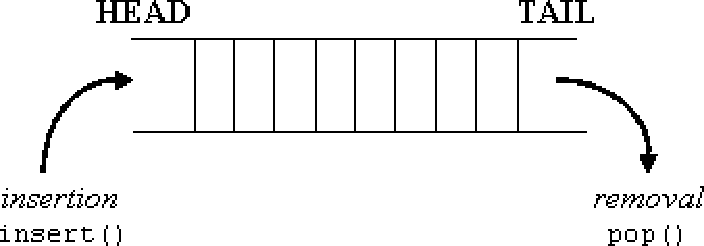
\includegraphics[width=3.703in, height=1.303in]{figures/usmanFig10}
    \caption{cQueue: insertion and removal}
    \label{fig:ch-sim-lib:cqueue}
  \end{center}
\end{figure}

The basic \cclass{cQueue} member functions dealing with insertion and removal
are \fname{insert()} and \fname{pop()}. They are used
like this:

\begin{verbatim}
cQueue queue("my-queue");
cMessage *msg;

// insert messages
for (int i=0; i<10; i++)
{
  msg = new cMessage;
  queue.insert( msg );
}

// remove messages
while( ! queue.empty() )
{
  msg = (cMessage *)queue.pop();
  delete msg;
}
\end{verbatim}


The \fname{length()} member function returns the number of items in the
queue, and \fname{empty()} tells whether there's anything in the queue.

There are other functions dealing with insertion and removal.  The
\fname{insertBefore()} and \fname{insertAfter()} functions insert a
new item exactly before and after a specified one, regardless of the
ordering function.

The \fname{tail()} and \fname{head()} functions return pointers to the objects
at the tail and head of the queue, without affecting queue contents.

The \fname{pop()} function can be used to remove items from the
tail of the queue, and the \fname{remove()} function can be
used to remove any item known by its pointer from the queue:

\begin{verbatim}
queue.remove( msg );
\end{verbatim}



\subsubsection{Priority queue}


By default, \cclass{cQueue} implements a FIFO, but it can also act as
a priority queue, that is, it can keep the inserted objects
ordered\index{queue!order}.  If you want to use this feature, you have
to provide a function that takes two \cclass{cObject} pointers,
compares the two objects and returns -1, 0 or 1 as the result (see the
reference for details).  An example of setting up an ordered
\cclass{cQueue}:

\begin{verbatim}
cQueue sortedqueue("sortedqueue", cObject::cmpbyname, true );
                        // sorted by object name, ascending
\end{verbatim}


If the queue object is set up as an ordered queue, the \fname{insert()}
function uses the ordering function: it searches the queue contents
from the head until it reaches the position where the new item
needs to be inserted, and inserts it there.


\subsubsection{Iterators}


Normally, you can only access the objects at the head or tail of the
queue. However, if you use an iterator class, \cclass{cQueue::Iterator},
you can examine each object in the queue\index{queue!iteration}.

The \cclass{cQueue::Iterator} constructor takes two arguments, the first
is the queue object and the second one specifies the initial position
of the iterator: 0=tail, 1=head. Otherwise it acts as any other
{\opp} iterator class: you can use the ++ and -- operators to advance
it, the () operator to get a pointer to the current item, and the
\fname{end()} member function to examine if you're at the end (or the
beginning) of the queue.


An example:

\begin{verbatim}
for( cQueue::Iterator iter(queue,1); !iter.end(), iter++)
{
  cMessage *msg = (cMessage *) iter();
  //...
}
\end{verbatim}




\subsection{Expandable array: cArray}

\subsubsection{Basic usage}


\cclass{cArray} is a container class that holds objects derived from
\cclass{cObject}. \cclass{cArray} stores the pointers of the objects
inserted instead of making copies. \cclass{cArray} works as an array,
but if it gets full, it grows automatically. Internally,
\cclass{cArray} is implemented with an array of pointers; if the array
gets full, it is reallocated.

\cclass{cArray} objects are used in {\opp} to store parameters
attached to messages, and internally, for storing module parameters
and gates.


Creating an array:

\begin{verbatim}
cArray array("array");
\end{verbatim}

Adding an object at the first free index:

\begin{verbatim}
cPar *p = new cPar("par");
int index = array.add( p );
\end{verbatim}


Adding an object at a given index (if the index is occupied,
you'll get an error message):

\begin{verbatim}
cPar *p = new cPar("par");
int index = array.addAt(5,p);
\end{verbatim}


Finding an object in the array:

\begin{verbatim}
int index = array.find(p);
\end{verbatim}

Getting a pointer to an object at a given index:

\begin{verbatim}
cPar *p = (cPar *) array[index];
\end{verbatim}

You can also search the array or get a pointer to an object by
the object's name:

\begin{verbatim}
int index = array.find("par");
Par *p = (cPar *) array["par"];
\end{verbatim}


You can remove an object from the array by calling \fname{remove()}
with the object name, the index position or the object pointer:

\begin{verbatim}
array.remove("par");
array.remove(index);
array.remove( p );
\end{verbatim}


The \fname{remove()} function doesn't deallocate the object, but it
returns the object pointer. If you also want to deallocate it, you can
write:

\begin{verbatim}
delete array.remove( index );
\end{verbatim}

\subsubsection{Iteration}


\cclass{cArray} has no iterator, but it's easy to loop through all the
indices with an integer variable. The \fname{items()} member function
returns the largest index plus one.

\begin{verbatim}
for (int i=0; i<array.items(); i++)
{
  if (array[i]) // is this position used?
  {
    cObject *obj = array[i];
    ev << obj->name() << endl;
  }
}
\end{verbatim}


%
% \section{Non-object container classes}
%
% There are two container classes to store non-object
% items\index{non-object container}: \cclass{cLinkedList} and
% \cclass{cBag}.  The first one parallels with \cclass{cQueue}, the
% second one with \cclass{cArray}. They can be useful if you have to
% deal with C structs or objects that are not derived from
% \cclass{cObject}.
%
% See the class library reference for more info about them.
%




\section{The parameter class: cPar}
\label{sec:ch-sim-lib:cpar}

Module parameters (as discussed in section \ref{ch:simple-modules:parameters})
are represented as \cclass{cPar} objects.
The module parameter name is the \cclass{cPar} object's name, and the object
can store any parameter type supported by the NED language, that is,
numeric (long or double), bool, string and XML config file reference.
    \footnote{\cclass{cPar} objects used to be employed also for adding
    parameters (extra fields) to \cclass{cMessage}. However, while technically this is
    still feasible, message definitions (section \ref{ch:messages:message-definitions})
    are a far superior solution in every respect.}

Module parameters are accessed via \cclass{cModule}'s \fname{par()} method:

\begin{verbatim}
cPar& par(const char *parameterName);
\end{verbatim}

\subsection{Reading the value}

\cclass{cPar} has a number of methods for getting the parameter's value:

\begin{verbatim}
bool boolValue();
long longValue();
const char *stringValue();
double doubleValue();
cXMLElement *xmlValue();
\end{verbatim}

There are also overloaded type cast operators for C/C++ primitive types
including \ttt{bool}, \ttt{int}, \ttt{long}, \ttt{double}, \ttt{const char *},
and also for \ttt{cXMLElement *}.
    \footnote{\cclass{cPar} also supports the \ttt{void *} and \ttt{cObject *} types,
    but these types were used primarily for message parameters before
    message definitions (section \ref{ch:messages:message-definitions})
    got supported, and you cannot create such module parameters from NED.}

Thus, any of the following ways would work to store a parameter's value in
a variable:

\begin{verbatim}
double foo = par("foo").doubleValue();
double foo = (double) par("foo");
double foo = par("foo");
\end{verbatim}

If you use the \ttt{par("foo")} parameter in expressions (such as
\ttt{4*par("foo")+2}), the C++ compiler may be unable to decide
between overloaded operators and report ambiguity. In that case
you have to clarify by adding either an explicit cast
(\ttt{(double)par("foo")} or \ttt{(long)par("foo")}) or use
the \ttt{doubleValue()} or \ttt{longValue()} methods.

\subsection{Changing the value}

There are many ways to set a \cclass{cPar}'s value. One is the \ttt{set...Value()}
member functions:

\begin{verbatim}
cPar& foo = par("foo");
foo.setLongValue(12);
foo.setDoubleValue(2.7371);
foo.setStringValue("one two three");
\end{verbatim}

There are also overloaded assignment operators for C++ primitive types,
\ttt{const char *}, and \ttt{cXMLElement *}.

\begin{verbatim}
cPar pp("pp");
pp = 12;
pp = 2.7371;
pp = "one two three";
\end{verbatim}

The \cclass{cPar} object makes its own copy of the string, so the
original one does not need to be preserved. Short strings (less than
\ensuremath{\sim}20 chars) are handled more efficiently because they
are stored in the object's memory space (and are not dynamically
allocated).

\cclass{cPar} can also store other types which yield numeric
results such as function with constant args;
they will be mentioned in the next section.

For numeric and string types, an input flag\index{input flag} can be
set. In this case, when the object's value is first used, the
parameter value will be searched for in the configuration (ini)
file\index{ini file}; if it is not found there, the user will be offered
to enter the value interactively.

Examples:

\begin{verbatim}
cPar foo("foo");
foo.setPrompt("Enter foo value:");
foo.setInput(true);   // make it an input parameter

double d = (double)foo; // the user will be prompted HERE
\end{verbatim}

\subsection{Setting cPar to return random numbers}

Setting \cclass{cPar} to call a function with constant arguments can
be used to make \cclass{cPar} return random variables\index{random!variables}
from different distributions\index{distribution}:

\begin{verbatim}
cPar rnd("rnd");
rnd.setDoubleValue(intuniform, -10.0, 10.0);// uniform distr.
rnd.setDoubleValue(normal, 100.0, 5.0); // normal distr. (mean,dev)
rnd.setDoubleValue(exponential, 10.0); // exponential distr. (mean)
\end{verbatim}

\fname{intuniform()}, \fname{normal()} etc. are ordinary C functions
taking double arguments and returning double. Each time you read the
value of a \cclass{cPar} containing a function like above, the
function will be called with the given constant arguments (e.g.
\ttt{normal(100.0,5.0)}) and its return value used.

The above functions use number 0 from the several random number
generators. To use another generator, use the \ttt{genk\_xxx} versions
of the random functions:

\begin{verbatim}
rnd.setDoubleValue(genk_normal, 3, 100.0, 5.0); // uses generator 3
\end{verbatim}

A \cclass{cPar} object can also be set to return a random variable from
a distribution collected by a statistical data collection object:

\begin{verbatim}
cDoubleHistogram hist =....; // the distribution
cPar rnd2("rnd2");
rnd2.setDoubleValue(hist);
\end{verbatim}


%
% \subsection{Storing object and non-object pointers in cPar}
% \subsection{Reverse Polish expressions}
% \subsection{Using redirection}
%
% These section got dumped in 3.0, they can be digged out from the CVS if needed.
%

\subsection{cPar storage types}

\cclass{cPar} supports the basic data types (long, double, bool, string, XML) via
several \textit{storage types}. Storage types are internally
identified by type characters. The type character is
returned by the \fname{type()} method.

Example:

\begin{verbatim}
cPar par = 10L;
char typechar = par.type(); // returns storage type 'L'
\end{verbatim}

The all \cclass{cPar} data types and are summarized in the table below.
The \fname{isNumeric()} function tells whether the object
stores a data types which allows the \fname{doubleValue()} method
to be called.

\begin{longtable}{|p{0.7cm}|p{1.2cm}|p{5.2cm}|p{6cm}|}
\hline
% ROW 1
\tabheadcol
\textbf{Type\linebreak char} &
\textbf{Storage\linebreak type} &
\textbf{Member functions} &
\textbf{Description}\\
\hline
%% ROW 2
S &  string &
\ttt{setStringValue( \linebreak
\hspace*{0.3cm}  const char *); \linebreak
const char * \linebreak
\hspace*{0.3cm} \fname{stringValue()}; \linebreak
op const char *(); \linebreak
op=(const char *);} &
{\raggedright
string value. Short strings (len\texttt{<}=27) are stored inside
\cclass{cPar} object, without using heap allocation.}\\\hline
%% ROW 3
B &  boolean &
\ttt{setBoolValue(bool); \linebreak
bool \fname{boolValue()}; \linebreak
op \fname{bool()}; \linebreak
op=(bool);} &
boolean value. Can also be retrieved from the object as long  (0 or 1).\\\hline
%% ROW 4
L & long int &
\ttt{setLongValue(long); \linebreak
long \fname{longValue()}; \linebreak
op \fname{long()}; \linebreak
op=(long);} &
signed long integer value. Can also be retrieved from the object
as double.\\\hline
%% ROW 5
D & double &
\ttt{setDoubleValue(double); \linebreak
double \fname{doubleValue()}; \linebreak
op \fname{double()}; \linebreak
op=(double);} &
double-precision floating point value.\\\hline
%% ROW 6
F & function &
\ttt{setDoubleValue( \linebreak
\hspace*{0.3cm} MathFunc, \linebreak
\hspace*{0.3cm} [double], \linebreak
\hspace*{0.3cm} [double], \linebreak
\hspace*{0.3cm} [double]); \linebreak
double \fname{doubleValue()}; \linebreak
op \fname{double()}; \linebreak
} &
Mathematical function with constant arguments. The function
is given by its pointer; it must take 0,1,2 or 3 doubles and
return a double. This type is mainly used to generate random
numbers: e.g. the function takes mean and standard deviation
and returns random variable of a certain distribution.\\\hline
%% ROW 7
X & expr. &
\ttt{setDoubleValue( \linebreak
\hspace*{0.3cm} cPar::ExprElem*,int); \linebreak
double \fname{doubleValue()}; \linebreak
op \fname{double()};}
&
Reverse Polish expression. Expression can contain constants,
\cclass{cPar} objects, refer to other \cclass{cPars} (e.g. module parameters),
can use many math operators (+-*/{\textasciicircum}\% etc), function calls
(function must take 0,1,2 or 3 doubles and return a double).
The expression must be given is in an cPar::ExprElem array (see later).\\\hline
%% ROW 8
T & distrib. &
\ttt{setDoubleValue( \linebreak
\hspace*{0.3cm} \cclass{cStatistic}*); \linebreak
double \fname{doubleValue()}; \linebreak
op \fname{double()}; \linebreak
} &
random variable generated from a distribution collected by a
statistical data collection object (derived from \cclass{cStatistic}).\\\hline
%% ROW 9
P & void* pointer &
\ttt{setPointerValue(void*); \linebreak
void *\fname{pointerValue()}; \linebreak
op void *(); \linebreak
op=(void *);} &
pointer to a non-\cclass{cObject} item (C struct, non-\cclass{cObject} object
etc.) Memory management can be controlled through the \fname{configPointer()}
member function.\\\hline
%% ROW 10
O & object pointer &
\ttt{setObjectValue(cObject*); \linebreak
cObject *\fname{objectValue()}; \linebreak
op cObject *(); \linebreak
op=(cObject *);}
&
{\raggedright pointer to an object derived from \cclass{cObject}.
Ownership management is done through \fname{takeOwnership()}.}\\\hline
%% ROW 11
I & indirect value &
\ttt{setRedirection(cPar*); \linebreak
bool \fname{isRedirected()}; \linebreak
cPar *\fname{redirection()}; \linebreak
\fname{cancelRedirection()};}
&
{\raggedright value is redirected to another \cclass{cPar} object. All value setting
and reading operates on the other \cclass{cPar}; even the \fname{type()} function
will return the type in the other \cclass{cPar} (so you'll never get 'I'
as the type). This redirection can only be broken with the \fname{cancelRedirection()}
member function. Module parameters taken by \ttt{ref} use this mechanism.}\\\hline
\end{longtable}





\section{Routing support: cTopology}

\subsection{Overview}

The \cclass{cTopology} class was designed primarily to support
routing\index{routing support} in telecommunication or multiprocessor
networks.

A \cclass{cTopology} object stores an abstract representation of the
network in graph form:
\begin{itemize}
  \item{each \cclass{cTopology} node corresponds to a \textit{module}
    (simple or compound), and}
  \item{each \cclass{cTopology} edge corresponds to a \textit{link} or
    \textit{series of connecting links}.}
\end{itemize}

You can specify which modules (either simple or compound) you want to
include in the graph. The graph will include all connections among the
selected modules. In the graph, all nodes are at the same level,
there's no submodule nesting.  Connections which span across compound
module boundaries are also represented as one graph edge. Graph edges
are directed, just as module gates are.


If you're writing a router or switch model, the \cclass{cTopology}
graph can help you determine what nodes are available through which
gate and also to find optimal routes\index{optimal routes}. The
\cclass{cTopology} object can calculate shortest paths\index{shortest
  path} between nodes for you.

The mapping between the graph (nodes, edges) and network model
(modules, gates, connections) is preserved: you can easily find
the corresponding module for a \cclass{cTopology} node and vica versa.





\subsection{Basic usage}

You can extract the network topology into a \cclass{cTopology}
object by a single function call. You have several ways to select
which modules you want to include in the topology:
\begin{itemize}
  \item{by module type}
  \item{by a parameter's presence and its value}
  \item{with a user-supplied boolean function}
\end{itemize}

First, you can specify which node types you want to include. The
following code extracts all modules of type Router or User. (Router
and User can be both simple and compound module types.)

\begin{verbatim}
cTopology topo;
topo.extractByModuleType( "Router", "User", NULL );
\end{verbatim}


Any number of module types (up to 32) can be supplied; the list
must be terminated by \ttt{NULL}.

Second, you can extract all modules which have a certain parameter:

\begin{verbatim}
topo.extractByParameter( "ipAddress" );
\end{verbatim}


You can also specify that the parameter must have a certain value
for the module to be included in the graph:

\begin{verbatim}
cPar yes = "yes";
topo.extractByParameter( "includeInTopo", &yes );
\end{verbatim}

The third form allows you to pass a function which can determine for
each module whether it should or should not be included.  You can have
\cclass{cTopology} pass supplemental data to the function through a
void* pointer. An example which selects all top-level modules (and
does not use the void* pointer):

\begin{verbatim}
int selectFunction(cModule *mod, void *)
{
  return mod->parentModule() == simulation.systemModule();
}

topo.extractFromNetwork( selectFunction, NULL );
\end{verbatim}

%
% TBD one more example which \textit{does use} the void* ptr.
%

A \cclass{cTopology} object uses two types: \cclass{sTopoNode} for
nodes and \cclass{sTopoLink} for edges. (\cclass{sTopo\-Link\-In} and
\cclass{sTopoLinkOut} are `aliases' for \cclass{sTopoLink}; we'll
talk about them later.)

Once you have the topology extracted, you can start exploring
it. Consider the following code (we'll explain it shortly):

\begin{verbatim}
for (int i=0; i<topo.nodes(); i++)
{
  sTopoNode *node = topo.node(i);
  ev << "Node i=" << i << " is " << node->module()->fullPath() << endl;
  ev << " It has " << node->outLinks() << " conns to other nodes\n";
  ev << " and " << node->inLinks() << " conns from other nodes\n";

  ev << " Connections to other modules are:\n";
  for (int j=0; j<node->outLinks(); j++)
  {
    sTopoNode *neighbour = node->out(j)->remoteNode();
    cGate *gate = node->out(j)->localGate();
    ev << " " << neighbour->module()->fullPath()
       << " through gate " << gate->fullName() << endl;
  }
}
\end{verbatim}

The \fname{nodes()} member function (1st line) returns the number of
nodes in the graph, and node(i) returns a pointer to the \textit{i}th
node, an \cclass{sTopoNode} structure.


The correspondence between a graph node and a module can be obtained
by:

\begin{verbatim}
sTopoNode *node = topo.nodeFor( module );
cModule *module = node->module();
\end{verbatim}


The \fname{nodeFor()} member function returns a pointer to the graph
node for a given module. (If the module is not in the graph, it
returns \ttt{NULL}). \fname{nodeFor()} uses binary search within the
\cclass{cTopology} object so it is fast enough.


\cclass{sTopoNode}'s other member functions let you determine the
connections of this node: \fname{inLinks()}, \fname{outLinks()} return
the number of connections, \ttt{in(i)} and
\ttt{out(i)} return pointers to graph edge objects.


By calling member functions of the graph edge object, you can
determine the modules and gates involved. The \fname{remoteNode()}
function returns the other end of the connection, and
\fname{localGate()}, \fname{remoteGate()}, \fname{localGateId()} and
\fname{remoteGateId()} return the gate pointers and ids of the gates
involved. (Actually, the implementation is a bit tricky here: the same
graph edge object \cclass{sTopoLink} is returned either as
\cclass{sTopoLinkIn} or as \cclass{sTopoLinkOut} so that ``remote''
and ``local'' can be correctly interpreted for edges of both
directions.)





\subsection{Shortest paths}

The real power of \cclass{cTopology} is in finding shortest
paths\index{topology!shortest path} in the network to support optimal
routing\index{optimal routing}. \cclass{cTopology} finds shortest paths
from \textit{all} nodes \textit{to} a target node. The algorithm is
computationally inexpensive. In the simplest case, all edges are
assumed to have the same weight.

A real-life example when we have the target module pointer, finding
the shortest path looks like this:

\begin{verbatim}
cModule *targetmodulep =...;
sTopoNode *targetnode = topo.nodeFor( targetmodulep );
topo.unweightedSingleShortestPathsTo( targetnode );
\end{verbatim}


This performs the Dijkstra algorithm\index{Dijkstra algorithm} and
stores the result in the \cclass{cTopology} object. The result can
then be extracted using \cclass{cTopology} and
\ttt{sTopoNode}\index{sTopoNode} methods.  Naturally, each call to
\fname{unweightedSingleShortestPathsTo()} overwrites the results of
the previous call.

Walking along the path from our module to the target node:

\begin{verbatim}
sTopoNode *node = topo.nodeFor( this );

if (node == NULL)
{
  ev < "We (" << fullPath() << ") are not included in the topology.\n";
}
else if (node->paths()==0)
{
  ev << "No path to destination.\n";
}
else
{
  while (node != topo.targetNode())
  {
    ev << "We are in " << node->module()->fullPath() << endl;
    ev << node->distanceToTarget() << " hops to go\n";
    ev << "There are " << node->paths()
       << " equally good directions, taking the first one\n";
    sTopoLinkOut *path = node->path(0);
    ev << "Taking gate " << path->localGate()->fullName()
       << " we arrive in " << path->remoteNode()->module()->fullPath()
       << " on its gate " << path->remoteGate()->fullName() << endl;
    node = path->remoteNode();
  }
}
\end{verbatim}


The purpose of the \fname{distanceToTarget()} member function of a
node is self-explanatory. In the unweighted case, it returns the
number of hops. The \fname{paths()} member function returns the number
of edges which are part of a shortest path, and
\fname[path()]{path(i)} returns the \textit{i}th edge of them as
\cclass{sTopoLinkOut}. If the shortest paths were created by the
\fname[SingleShortestPaths()]{...SingleShortestPaths()} function,
\fname{paths()} will always return 1 (or 0 if the target is not
reachable), that is, only one of the several possible shortest paths
are found.  The
\fname[MultiShortestPathsTo()]{...MultiShortestPathsTo()} functions
find all paths, at increased run-time cost. The \cclass{cTopology}'s
\fname{targetNode()} function returns the target node of the last
shortest path search.

You can enable/disable nodes or edges in the graph. This is done by
calling their \fname{enable()} or \fname{disable()} member functions.
Disabled nodes or edges are ignored by the shortest paths calculation
algorithm. The \fname{enabled()} member function returns the state of
a node or edge in the topology graph.

One usage of \fname{disable()} is when you want to determine in how many
hops the target node can be reached from our node \textit{through
a particular output gate}. To calculate this, you calculate the
shortest paths to the target \textit{from the neighbor node}, but
you must disable the current node to prevent the shortest paths
from going through it:

\begin{verbatim}
sTopoNode *thisnode = topo.nodeFor( this );
thisnode->disable();
topo.unweightedSingleShortestPathsTo( targetnode );
thisnode->enable();

for (int j=0; j<thisnode->outLinks(); j++)
{
  sTopoLinkOut *link = thisnode->out(i);
  ev << "Through gate " << link->localGate()->fullName() << " : "
     << 1 + link->remoteNode()->distanceToTarget() << " hops" << endl;
}
\end{verbatim}

In the future, other shortest path algorithms will also be implemented:

\begin{verbatim}
unweightedMultiShortestPathsTo(sTopoNode *target);
weightedSingleShortestPathsTo(sTopoNode *target);
weightedMultiShortestPathsTo(sTopoNode *target);
\end{verbatim}






\section{Statistics and distribution estimation}

\subsection{cStatistic and descendants}

There are several statistic and result collection classes:
\cclass{cStdDev}, \cclass{cWeightedStdDev}, \cclass{Long\-Histogram},
\cclass{cDoubleHistogram}, \cclass{cVarHistogram}, \cclass{cPSquare} and
\cclass{cKSplit}. They are all derived from the abstract base class
\cclass{cStatistic}.

\begin{itemize}
  \item{\cclass{cStdDev} keeps number of samples, mean, standard
    deviation, minimum and maximum value etc.}
  \item{\cclass{cWeightedStdDev} is similar to \cclass{cStdDev}, but
    accepts weighted observations. \cclass{cWeightedStdDev} can be used
    for example to calculate time average. It is the only weighted
    statistics class.}
  \item{\cclass{cLongHistogram} and \cclass{cDoubleHistogram} are
    descendants of \cclass{cStdDev} and also keep an approximation of
    the distribution of the observations using equidistant
    (equal-sized) cell histograms\index{histogram!equal-sized}.}
  \item{\cclass{cVarHistogram} implements a histogram where cells do not
    need to be the same size. You can manually add the cell (bin)
    boundaries, or alternatively, automatically have a partitioning
    created where each bin has the same number of observations (or as
    close to that as possible).}
  \item{\cclass{cPSquare} is a class that uses the $P^{2}$ algorithm
    described in \cite{JCh85}. The algorithm calculates quantiles without
    storing the observations; one can also think of it as a histogram
    with equiprobable cells\index{histogram!equiprobable-cells}.}
  \item{\cclass{cKSplit} uses a novel, experimental method, based on an
    adaptive histogram-like algorithm.}
\end{itemize}

\subsubsection{Basic usage}

One can insert an observation into a statistic object with the
\fname{collect()} function or the \texttt{+=} operator (they are
equivalent).  \cclass{cStdDev} has the following methods for getting
statistics out of the object: \fname{samples()}, \fname{min()},
\fname{max()}, \fname{mean()}, \fname{stddev()}, \fname{variance()},
\fname{sum()}, \fname{sqrSum()} with the obvious meanings. An example
usage for \cclass{cStdDev}:

\begin{verbatim}
cStdDev stat("stat");

for (int i=0; i<10; i++)
  stat.collect( normal(0,1) );

long numSamples = stat.samples();
double smallest = stat.min(),
       largest = stat.max();
double mean = stat.mean(),
       standardDeviation = stat.stddev(),
       variance = stat.variance();
\end{verbatim}





\subsection{Distribution estimation}

\subsubsection{Initialization and usage}


The distribution estimation\index{distribution!estimation} classes (the histogram classes,
\cclass{cPSquare} and \cclass{cKSplit}) are derived from
\cclass{cDensityEstBase}. Distribution estimation classes (except for
\cclass{cPSquare}) assume that the observations are within a range.
You may specify the range explicitly (based on some a-priori info
about the distribution) or you may let the object collect the first
few observations and determine the range from them. Methods which let
you specify range settings are part of \cclass{cDensityEstBase}.

The following member functions exist for setting up the range
and to specify how many observations should be used for
automatically determining the range.

\begin{verbatim}
setRange(lower,upper);
setRangeAuto(numFirstvals, rangeExtFactor);
setRangeAutoLower(upper, numFirstvals, rangeExtFactor);
setRangeAutoUpper(lower, num, rangeExtFactor);
\end{verbatim}

\begin{verbatim}
setNumFirstVals(numFirstvals);
\end{verbatim}

The following example creates a histogram with 20 cells and automatic
range estimation\index{histogram!range estimation}:

\begin{verbatim}
cDoubleHistogram histogram("histogram", 20);
histogram.setRangeAuto(100,1.5);
\end{verbatim}


Here, 20 is the number of cells (not including the underflow/overflow
cells, see later), and 100 is the number of observations to be
collected before setting up the cells. 1.5 is the range extension
factor. It means that the actual range of the initial observations
will be expanded 1.5 times and this expanded range will be used to lay
out the cells. This method increases the chance that further
observations fall in one of the cells and not outside the histogram
range.

\begin{figure}[htbp]
  \begin{center}
    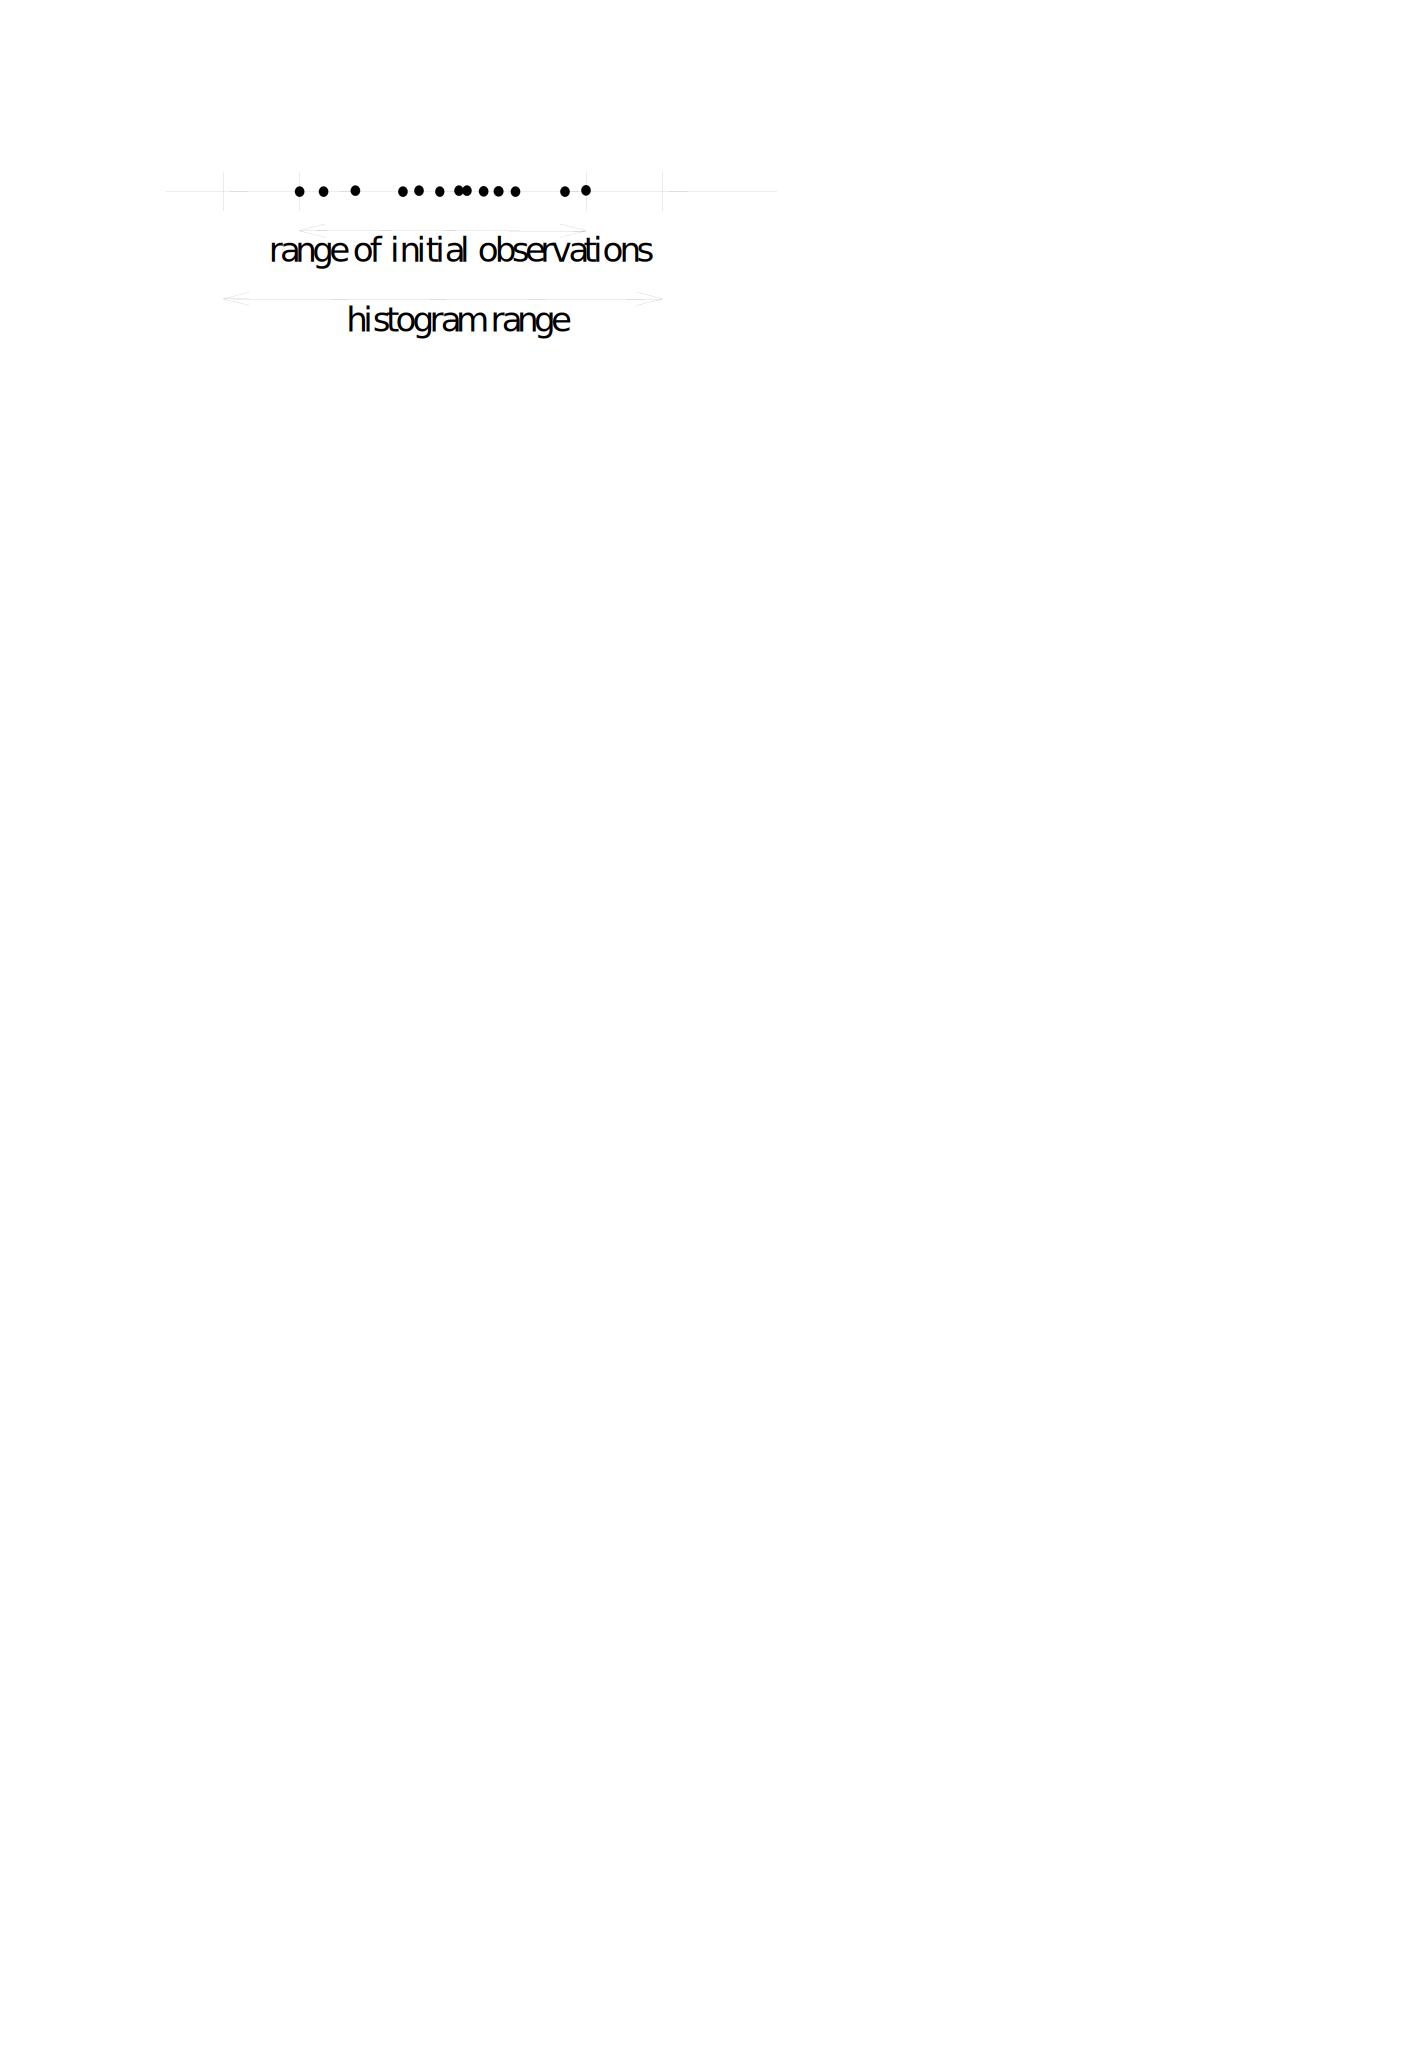
\includegraphics[width=3.215in, height=0.930in]{figures/usmanFig12}
    \caption{Setting up a histogram's range}
  \end{center}
\end{figure}

After the cells have been set up, collecting can go on.

The \fname{transformed()} function returns \textit{true} when the cells have
already been set up. You can force range estimation and setting
up the cells by calling the \fname{transform()} function.

The observations that fall outside the histogram range will be counted
as underflows and overflows. The number of underflows and overflows
are returned by the \fname{underflowCell()} and \fname{overflowCell()}
member functions.

\begin{figure}[htbp]
\begin{center}
  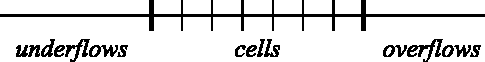
\includegraphics[width=3.310in, height=0.467in]{figures/usmanFig13}
  \caption{Histogram structure after setting up the cells}
\end{center}
\end{figure}

You create a $P^{2}$ object by specifying the number of cells:

\begin{verbatim}
cPSquare psquare("interarrival-times", 20);
\end{verbatim}

Afterwards, a \cclass{cPSquare} can be used with the same member functions
as a histogram.


\subsubsection{Getting histogram data}


There are three member functions to explicitly return cell boundaries
and the number of observations is each cell. \fname{cells()} returns
the number of cells, \fname[basepoint()]{basepoint(int k)} returns the
\textit{k}th base point, \fname[cell()]{cell(int k)} returns the
number of observations in cell \textit{k}, and
\fname[cellPDF()]{cellPDF(int k)} returns the PDF value in the cell
(i.e. between \fname[basepoint()]{basepoint(k)} and
\fname[basepoint()]{basepoint(k+1)}).  These functions work for all
histogram types, plus \cclass{cPSquare} and \cclass{cKSplit}.

\begin{figure}[htbp]
  \begin{center}
    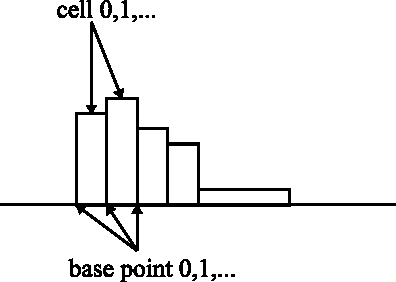
\includegraphics[width=2.615in, height=2.001in]{figures/usmanFig14}
    \caption{base points and cells}
  \end{center}
\end{figure}

An example:

\begin{verbatim}
long n = histogram.samples();
for (int i=0; i<histogram.cells(); i++)
{
  double cellWidth = histogram.basepoint(i+1)-histogram.basepoint(i);
  int count = histogram.cell(i);
  double pdf = histogram.cellPDF(i);
  //...
}
\end{verbatim}


The \fname[pdf()]{pdf(x)} and \fname[cdf()]{cdf(x)} member functions
return the value of the probability density function and the cumulated
density function at a given \textit{x}, respectively.


\subsubsection{Random number generation from distributions}


The \fname{random()} member function generates random
numbers\index{random!numbers} from the distribution stored by the
object:

\begin{verbatim}
double rnd = histogram.random();
\end{verbatim}


\cclass{cStdDev} assumes normal distribution.

You can also wrap the distribution object in a \cclass{cPar}:

\begin{verbatim}
cPar rndPar("rndPar");
rndPar.setDoubleValue(&histogram);
\end{verbatim}


The \cclass{cPar} object stores the pointer to the histogram (or $P^{2}$ object),
and whenever it is asked for the value, calls the histogram object's \fname{random()}
function:

\begin{verbatim}
double rnd = (double)rndPar; // random number from the cPSquare
\end{verbatim}

\subsubsection{Storing/loading distributions}


The statistic classes have \fname{loadFromFile()} member functions
that read the histogram data from a text file. If you need a custom
distribution\index{distribution!custom} that cannot be written (or it
is inefficient) as a C function, you can describe it in histogram form
stored in a text file, and use a histogram object with
\fname{loadFromFile()}.

You can also use \fname{saveToFile()}that writes out the distribution
collected by the histogram object:

\begin{verbatim}
FILE *f = fopen("histogram.dat","w");
histogram.saveToFile( f ); // save the distribution
fclose( f );

FILE *f2 = fopen("histogram.dat","r");}
cDoubleHistogram hist2("Hist-from-file");
hist2.loadFromFile( f2 ); // load stored distribution
fclose( f2 );
\end{verbatim}


\subsubsection{Histogram with custom cells}


The \cclass{cVarHistogram} class can be used to create
histograms with arbitrary (non-equidistant) cells.
It can operate in two modes:

\begin{itemize}
  \item \textit{manual}, where you specify cell boundaries explicitly
     before starting collecting
  \item \textit{automatic}, where \fname{transform()} will set up the cells
     after collecting a certain number of initial observations. The cells
     will be set up so that as far as possible, an equal number of observations
     fall into each cell (equi-probable cells).
\end{itemize}

Modes are selected with a \textit{transform-type} parameter:
\begin{itemize}
  \item{\ttt{HIST\_TR\_NO\_TRANSFORM}: no transformation; uses bin boundaries
    previously defined by \fname{addBinBound()}}
  \item{\ttt{HIST\_TR\_AUTO\_EPC\_DBL}: automatically creates equiprobable cells}
  \item{\ttt{HIST\_TR\_AUTO\_EPC\_INT}: like the above, but for integers}
\end{itemize}

Creating an object:

\begin{verbatim}
cVarHistogram(const char *s=NULL,
              int numcells=11,
              int transformtype=HIST_TR_AUTO_EPC_DBL);
\end{verbatim}

Manually adding a cell boundary:

\begin{verbatim}
void addBinBound(double x);
\end{verbatim}

Rangemin and rangemax is chosen after collecting the
\texttt{numFirstVals} initial observations. One cannot add cell
boundaries when the histogram has already been transformed.





\subsection{The k-split algorithm}

\subsubsection{Purpose}


The \textit{k}-split algorithm is an on-line distribution
estimation\index{distribution!online estimation} method.  It was
designed for on-line result collection in simulation programs.  The
method was proposed by Varga and Fakhamzadeh in 1997. The primary
advantage of \textit{k}-split is that without having to store the
observations, it gives a good estimate without requiring a-priori
information about the distribution, including the sample size. The
\textit{k}-split algorithm can be extended to multi-dimensional
distributions\index{distribution!multi-dimensional}, but here we deal
with the one-dimensional version only.


\subsubsection{The algorithm}


The \textit{k-split} algorithm is an adaptive histogram-type estimate which
maintains a good partitioning by doing cell splits. We start out with
a histogram range $[x_{lo}, x_{hi})$ with $k$ equal-sized histogram
cells with observation counts $n_1,n_2, \cdots n_k$.  Each collected
observation increments the corresponding observation count. When an
observation count $n_i$ reaches a \textit{split threshold}, the cell
is split into $k$ smaller, equal-sized cells with observation counts
$n_{i,1}, n_{i,2}, \cdots n_{i,k}$ initialized to zero. The $n_i$
observation count is remembered and is called the \textit{mother
  observation count} to the newly created cells. Further observations
may cause cells to be split further (e.g. $n_{i,1,1},...n_{i,1,k}$
etc.), thus creating a $k$-order tree of observation counts where
leaves contain live counters that are actually incremented by new
observations, and intermediate nodes contain mother observation counts
for their children. If an observation falls outside the histogram
range, the range is extended in a natural manner by inserting new
level(s) at the top of the tree. The fundamental parameter to the
algorithm is the split factor $k$. Experience shows that $k=2$ worked best.

\begin{figure}[htbp]
  \begin{center}
    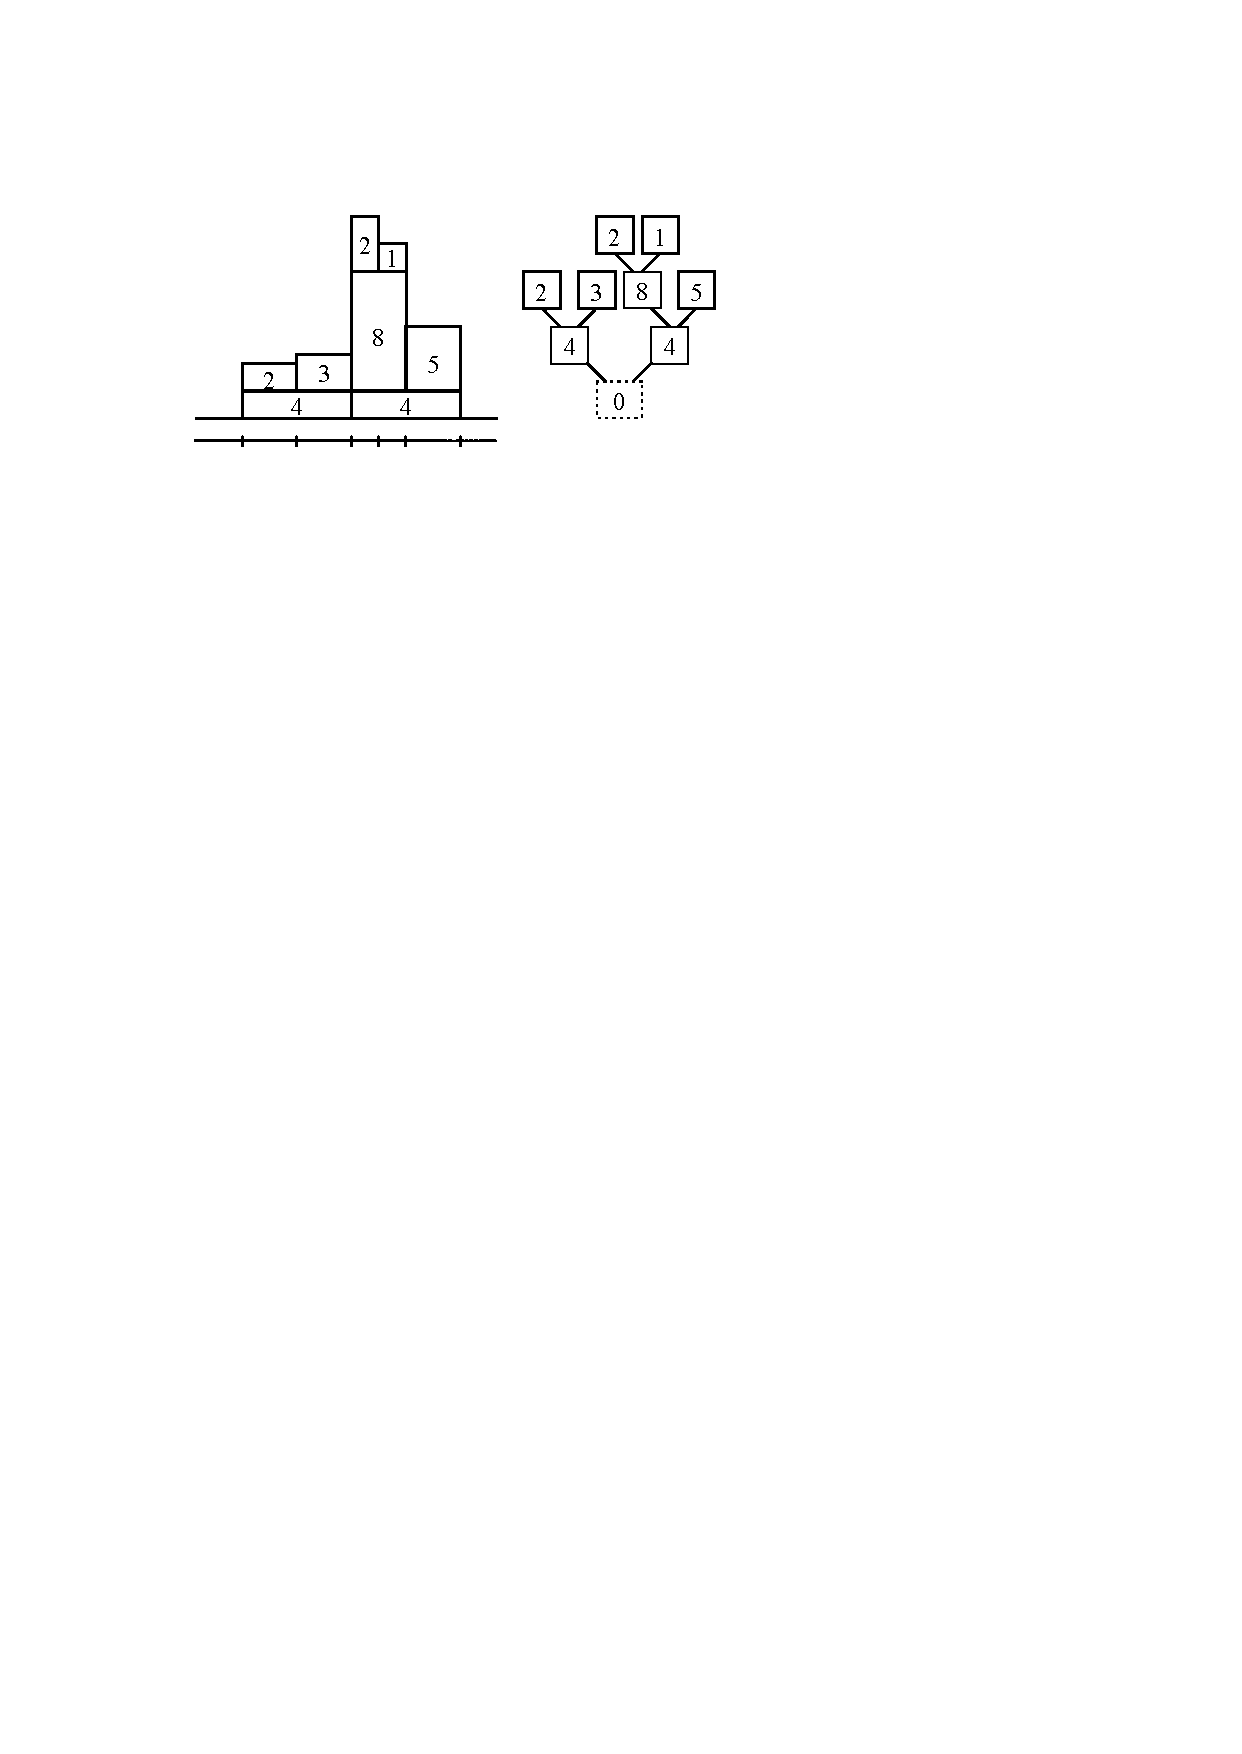
\includegraphics[width=3.442in, height=1.518in]{figures/usmanFig15}
    \caption{Illustration of the k-split algorithm, $k=2$. The
      numbers in boxes represent the observation count values}
  \end{center}
\end{figure}


For density estimation, the total number of observations that
fell into each cell of the partition has to be determined. For
this purpose, mother observations in each internal node of the
tree must be distributed among its child cells and propagated
up to the leaves.

% careful with reformatting! $..$ MUST NOT BE BROKEN TO SEVERAL LINES!

Let $n_{...,i}$ be the (mother) observation count for a cell,
$s_{...,i}$ be the total observation count in a cell $n_{...,i}$ plus
the observation counts in all its sub-, sub-sub-, etc. cells), and
$m_{...,i}$ the mother observations propagated to the cell. We are
interested in the $\tilde{n}_{...,i} = n_{...,i} + m_{...,i}$
estimated amount of observations in the tree nodes, especially in the
leaves. In other words, if we have $\tilde{n}_{...,i}$ estimated
observation amount in a cell, how to divide it to obtain
$m_{...,i,1}, m_{...,i,2} \cdots m_{...,i,k}$
that can be propagated to child cells. Naturally,
$m_{...,i,1} + m_{...,i,2} + \cdots + m_{...,i,k} = \tilde{n}_{...,i}$.

% careful with reformatting! $..$ MUST NOT BE BROKEN TO SEVERAL LINES!

Two natural distribution methods are even
distribution\index{distribution!even} (when
$m_{...,i,1} = m_{...,i,2} = \cdots = m_{...,i,k}$) and proportional
distribution\index{distribution!proportional} (when
$m_{...,i,1} : m_{...,i,2} : \cdots : m_{...,i,k} = s_{...,i,1} : s_{...,i,2} : \cdots : s_{...,i,k}$).
Even distribution is optimal when the
$s_{...,i,j}$ values are very small, and proportional distribution is
good when the $s_{...,i,j}$ values are large compared to
$m_{...,i,j}$. In practice, a linear combination of them seems
appropriate, where $\lambda=0$ means even and $\lambda=1$ means
proportional distribution:

% careful with reformatting! $..$ MUST NOT BE BROKEN TO SEVERAL LINES!

$m_{\cdots,i,j} = (1-\lambda)\tilde{n}_{\cdots,i}/k + \lambda \tilde{n}_{\cdots,i} s_{...,i,j} / s_{\cdots,i}$
where $\lambda\in[0,1]$

\begin{figure}[htbp]
  \begin{center}
    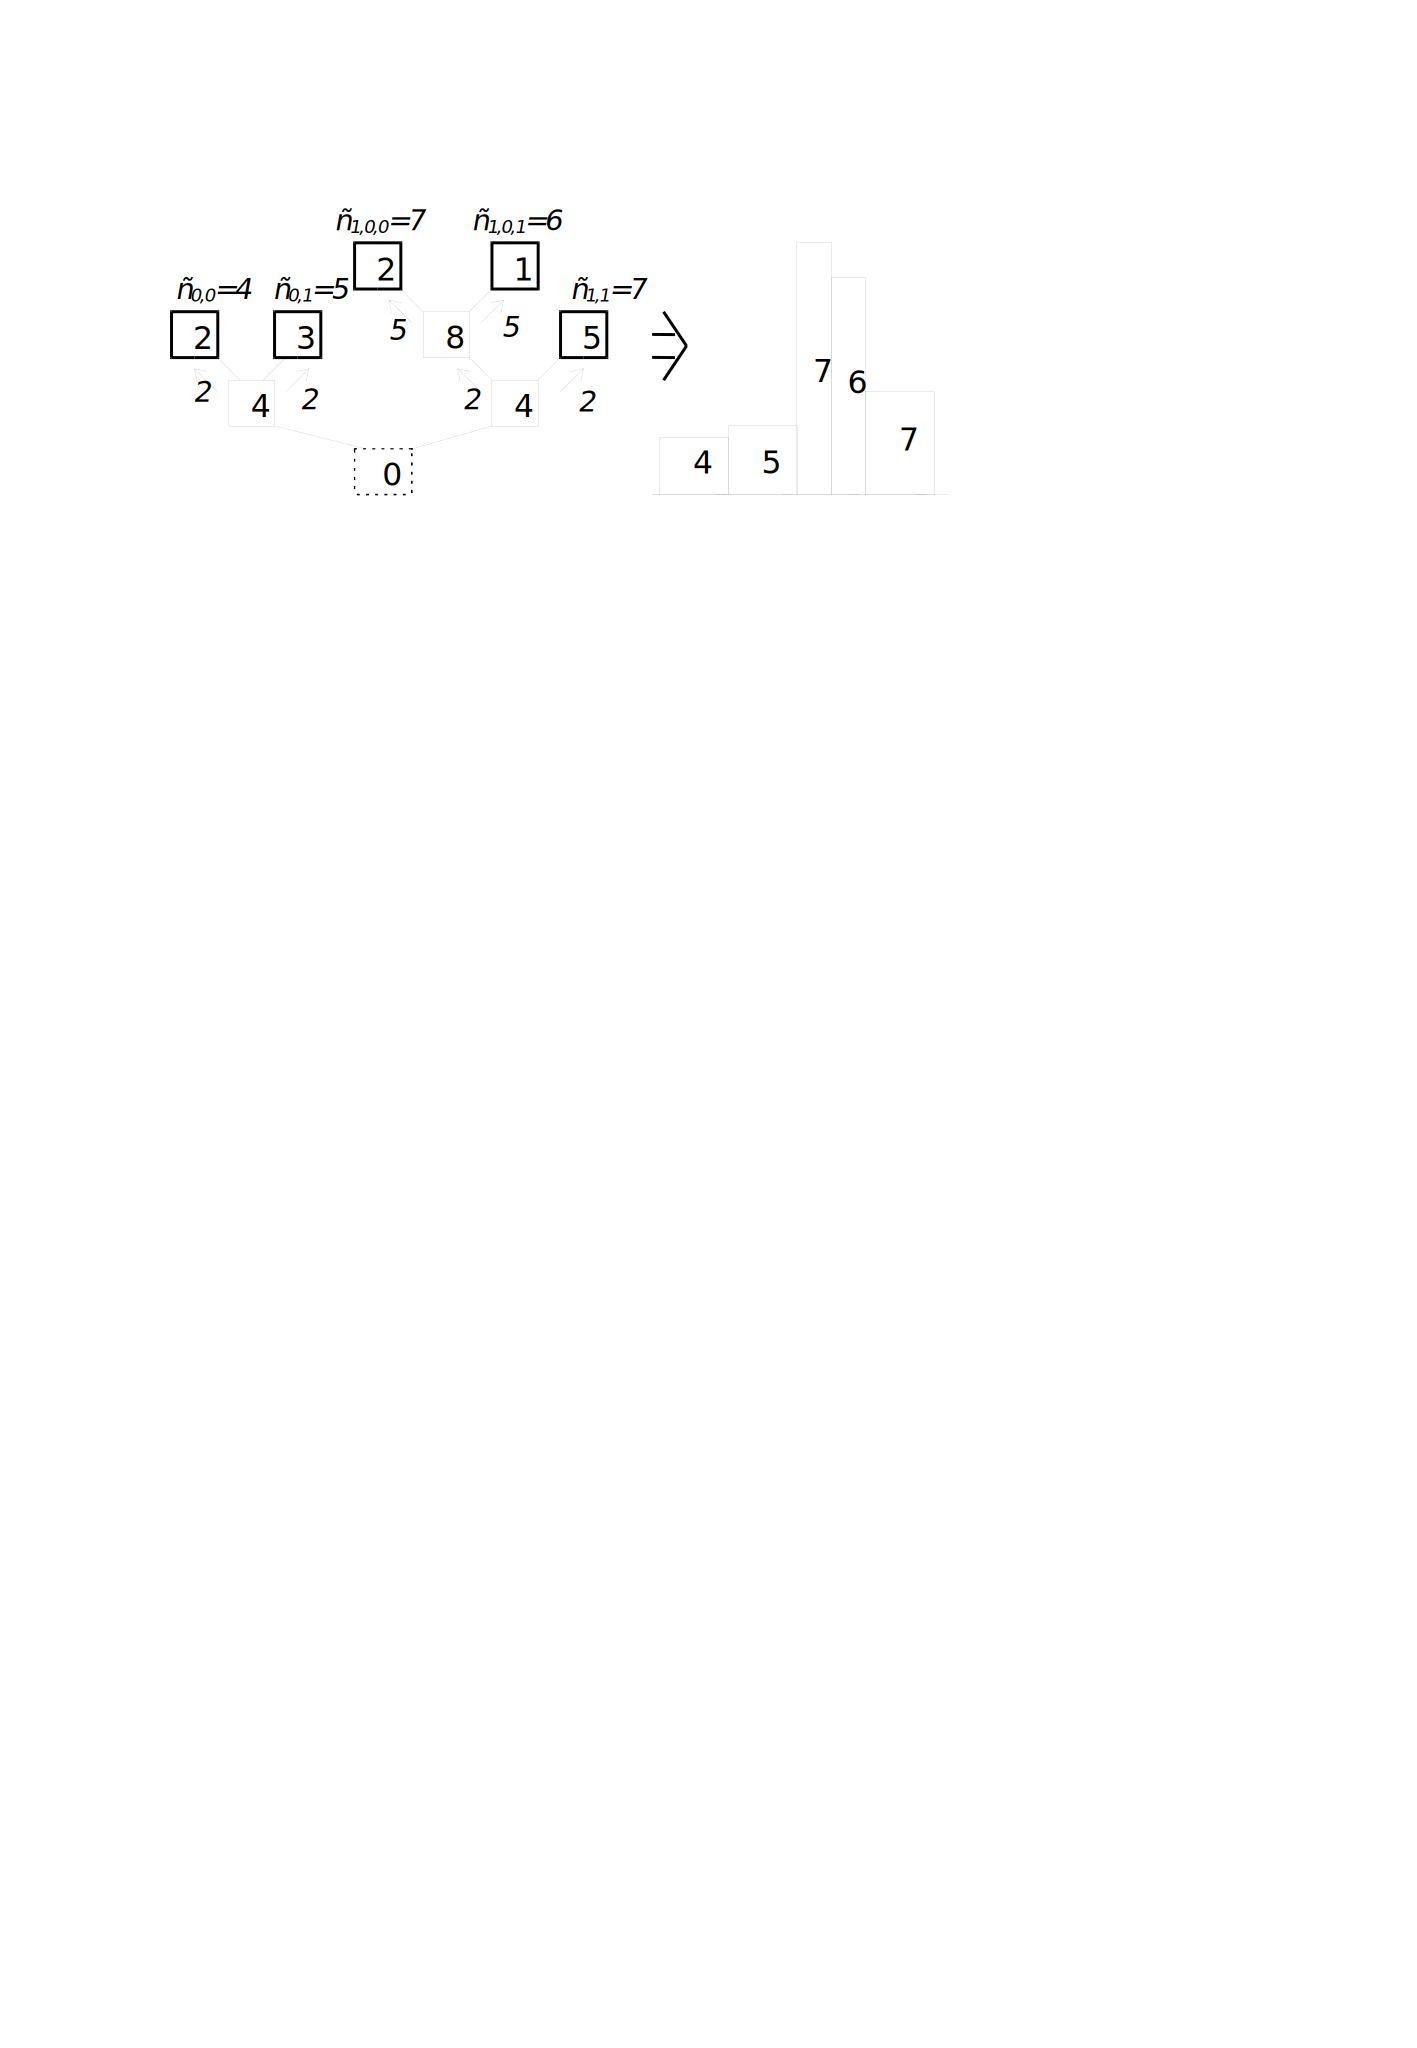
\includegraphics[width=4.147in, height=1.567in]{figures/usmanFig16}
    \caption{Density estimation from the k-split cell tree. We
      assume $\lambda=0$, i.e. we distribute mother observations
      evenly.}
  \end{center}
\end{figure}

% careful with reformatting! $..$ MUST NOT BE BROKEN TO SEVERAL LINES!

Note that while $n_{...,i}$ are integers, $m_{...,i}$ and thus
$\tilde{n}_{...,i}$ are typically real numbers. The histogram estimate
calculated from \textit{k}-split is not exact, because the frequency
counts calculated in the above manner contain a degree of estimation
themselves. This introduces a certain \textit{cell division error};
the $\lambda$ parameter should be selected so that it minimizes that
error. It has been shown that the cell division error can
be reduced to a more-than-acceptable small value.\\
Strictly speaking, the \textit{k}-split algorithm is semi-online,
because its needs some observations to set up the initial histogram
range.  However, because of the range extension and cell split
capabilities, the algorithm is not very sensitive to the choice of the
initial range, so very few observations are enough for range
estimation (say $N_{pre}=10$). Thus we can regard \textit{k}-split as
an on-line method.

\textit{K}-split can also be used in semi-online mode, when the
algorithm is only used to create an optimal partition from a larger
number of $N_{pre}$ observations. When the partition has been created,
the observation counts are cleared and the $N_{pre}$ observations are
fed into \textit{k}-split once again. This way all mother (non-leaf)
observation counts will be zero and the cell division error is
eliminated. It has been shown that the partition created by
\textit{k}-split can be better than both the equi-distant and the
equal-frequency partition.


{\opp} contains an experimental implementation of the \textit{k}-split
algorithm, the \cclass{cKSplit} class. Research on \textit{k}-split is
still under way.


\subsubsection{The cKSplit class}

The \cclass{cKSplit} class is an implementation of the \textit{k-split} method.
Member functions:

%
% TBD comments
%

\begin{verbatim}
void setCritFunc(KSplitCritFunc _critfunc, double *_critdata);
void setDivFunc(KSplitDivFunc \_divfunc, double *\_divdata);
void rangeExtension( bool enabled );
\end{verbatim}


\begin{verbatim}
int treeDepth();
int treeDepth(sGrid& grid);
\end{verbatim}

\begin{verbatim}
double realCellValue(sGrid& grid, int cell);
void printGrids();
\end{verbatim}

\begin{verbatim}
sGrid& grid(int k);
sGrid& rootGrid();
\end{verbatim}

\begin{verbatim}
struct sGrid
{
  int parent;   // index of parent grid
  int reldepth; // depth = (reldepth - rootgrid's reldepth)
  long total;   // sum of cells & all subgrids (includes `mother')
  int mother;   // observations `inherited' from mother cell
  int cells[K]; // cell values
};
\end{verbatim}



\subsection{Transient detection and result accuracy}

In many simulations, only the steady state performance (i.e.
the performance after the system has reached a stable state)
is of interest. The initial part of the simulation is called
the transient period. After the model has entered steady state,
simulation must proceed until enough statistical data have been
collected to compute result with the required accuracy.


Detection of the end of the transient period and a certain result
accuracy is supported by {\opp}. The user can attach transient
detection\index{transient detection} and result accuracy\index{result
  accuracy} objects to a result object (\cclass{cStatistic}'s
descendants). The transient detection and result accuracy objects will
do the specific algorithms on the data fed into the result object and
tell if the transient period is over or the result accuracy has been
reached.

The base classes for classes implementing specific transient
detection and result accuracy detection algorithms are:
\begin{itemize}
\item{\cclass{cTransientDetection}: base class for transient detection}
\item{\cclass{cAccuracyDetection}: base class for result accuracy detection}
\end{itemize}


\subsubsection{Basic usage}

%
% TBD comments
%

Attaching detection objects to a \cclass{cStatistic} and getting pointers
to the attached objects:

\begin{verbatim}
addTransientDetection(cTransientDetection *object);
addAccuracyDetection(cAccuracyDetection *object);
cTransientDetection *transientDetectionObject();
cAccuracyDetection *accuracyDetectionObject();
\end{verbatim}


Detecting the end of the period:
\begin{itemize}
\item{polling the \fname{detect()} function of the object}
\item{installing a post-detect function}
\end{itemize}


\subsubsection{Transient detection}


Currently one transient detection\index{transient detection} algorithm
is implemented, i.e.  there's one class derived from
\cclass{cTransientDetection}. The \cclass{cTDExpandingWindows} class
uses the sliding window approach with two windows, and checks the
difference of the two averages to see if the transient period is over.

\begin{verbatim}
void setParameters(int reps=3,
                   int minw=4,
                   double wind=1.3,
                   double acc=0.3);
\end{verbatim}

\subsubsection{Accuracy detection}


Currently one accuracy detection\index{accuracy detection} algorithm
is implemented, i.e.  there's one class derived from
\cclass{cAccuracyDetection}. The algorithm implemented in the
\cclass{cADByStddev} class is: divide the standard deviation by the
square of the number of values and check if this is small enough.

\begin{verbatim}
void setParameters(double acc=0.1, int reps=3);
\end{verbatim}




\section{Recording simulation results}

\subsection{Output vectors: cOutVector}
\label{sec:ch-sim-lib:coutvector}

Objects of type \cclass{cOutVector} are responsible for writing time series
data (referred to as \textit{output vectors}) to a file. The \fname{record()}
member is used to output a value (or a value pair) with a timestamp.

It can be used like this:

\begin{verbatim}
cOutVector respV("response time");

while (...)
{
  double responseTime;
  //...
  respV.record( responseTime );
  //...
}
\end{verbatim}


All \cclass{cOutVector} objects write to the same, common file. The
file is textual; each \fname{record()} call generates a line in the
file. The output file can be processed using Plove, but otherwise its
simple format allows it to be easily processed with \fprog{sed},
\fprog{awk}, \fprog{grep} and the like, and it can be imported by
spreadsheet programs.  The file format is described later in this
manual (in the section about simulation execution).

You can disable the output vector\index{output!vector} or specify a
simulation time interval for recording either from the ini file or
directly from program code:

\begin{verbatim}
cOutVector v("v");
simtime_t t =...;

v.enable();
v.disable();
v.setStartTime( t );
v.setStopTime( t+100.0 );
\end{verbatim}


If the output vector object is disabled or the simulation time is
outside the specified interval, \fname{record()} doesn't write
anything to the output file. However, if you have a Tkenv inspector
window open for the output vector object\index{output!vector object},
the values will be displayed there, regardless of the state of the
output vector object.





\subsection{Output scalars}

While output vectors are to record time series data and thus they
typically record a large volume of data during a simulation run,
output scalars\index{output!scalars} are supposed to record a single
value per simulation run. You can use outputs scalars
\begin{itemize}
\item{to record summary data at the end of the simulation run}
\item{to do several runs with different parameter settings/random seed
    and determine the dependence of some measures on the parameter
    settings. For example, multiple runs and output scalars are the
    way to produce \textit{Throughput vs. Offered Load} plots.}
\end{itemize}

Output scalars are recorded with the \fname{recordScalar()} member
function.  It is overloaded, you can use it to write doubles and
strings (const char *):

\begin{verbatim}
double avgThroughput = totalBits / simTime();
recordScalar("Average throughput", avgThroughput);
\end{verbatim}

You can record whole statistics objects by calling \fname{recordStats()}:

\begin{verbatim}
cStdDev *eedstats = new cStdDev;
...
recordStats("End-to-end Statistics", eedstats);
\end{verbatim}

Calls to \fname{recordScalar()} and \fname{recordStats()} are usually
placed in the redefined \fname{finish()} member function of a
simple module.

The above calls write into the (textual) output scalar file.  The
output scalar file is preserved across simulation runs (unlike the
output vector file is, scalar files are not deleted at the beginning
of each run). Data are always appended at the end of the file, and
output from different simulation runs are separated by special lines.




\section{Tracing and debugging aids}

\subsection{Displaying information about module activity}

You can have simple modules print textual output for
debugging\index{debugging} purposes.

The global object called \ttt{ev} represents the user interface of the
simulation program. You can send data to \ttt{ev}\index{ev} using the
C++-style I/O operator (\ttt{<}\ttt{<}).

\begin{verbatim}
ev << "started\n";
ev << "about to send message #" <<  i << endl;
ev << "queue full, discarding packet\n";
\end{verbatim}

The more traditional-looking but functionally equivalent
\fname{ev.printf()} form also exists.

\begin{verbatim}
ev.printf("%d packets dropped out of %d\n", drops, total);
\end{verbatim}

The exact way messages are displayed to the user depends on the user
interface. In the command-line user interface (Cmdenv\index{Cmdenv}),
it is simply dumped to the standard output. (This output can also be
disabled from the ini file so that it doesn't slow down simulation
when it is not needed.) In windowing user interfaces
(Tkenv\index{Tkenv}), each simple module can have
a separate text output window.

The above means that you should \textit{not} use \fname{printf()},
\fname{cout} \fname{<<} and the like because with Tkenv, their output
would appear in the terminal window behind the graphical window of the
simulation application.


\subsection{Watches}

You may want some of your int, long, double, char, etc. variables to
be inspect-able in Tkenv and to be output into the snapshot
file\index{snapshot file}. In this case, you can create
\cclass{cWatch} objects for them with the \fmac{WATCH()} macro:

\begin{verbatim}
int i; WATCH(i);
char c; WATCH(c);
\end{verbatim}

When you open an inspector for the simple module in Tkenv and click
the Objects/Watches tab in it, you'll see your WATCHed variables
and their values there. Tkenv also lets you change the value of a
WATCHed variable.

The \fmac{WATCH()} macro expands to a dynamically created \cclass{cWatch}
object.  The object remembers the address and type of your variable.
The macro expands to something like:

\begin{verbatim}
new cWatch("i",i);
\end{verbatim}


You can also make a \texttt{WATCH} for pointers of type \ttt{char*} or
\cclass[cObject]{cObject*}, but this may cause a segmentation fault if
the pointer does not point to a valid location when Tkenv or
\fname{snapshot()} wants to use it.

You can also set watches for variables that are members of the
module class\index{module!watches} or for structure fields:

\begin{verbatim}
WATCH( lapbconfig.timeout );
\end{verbatim}


\subsubsection{Placement of WATCHes}


Be careful not to execute a \fmac{WATCH()} statement more than once,
as each call would create a new \cclass{cWatch} object! If you use
\fname{activity()}, the best place for WATCHes is the top of the
\fname{activity()} function.  If you use \fname{handleMessage()},
place the \fname{WATCH()} statement into \fname{initialize()}.
\fname{WATCH()} creates a dynamic \cclass{cWatch} object, and we do
not want to create a new object each time \fname{handleMessage()} is
called.



\subsection{Snapshots}
\label{sec:ch-sim-lib:snapshots}

The \fname{snapshot()} function outputs textual information about all
or selected objects of the simulation (including the objects created
in module functions by the user) into the snapshot file\index{snapshot file}.

\begin{verbatim}
bool snapshot(cObject *obj = &simulation, const char *label = NULL);
\end{verbatim}


The function can be called from module functions, like this:

\begin{verbatim}
snapshot();     // dump the whole network
snapshot(this); // dump this simple module and all its objects
snapshot(&simulation.msgQueue); // dump future events
\end{verbatim}

This will append snapshot information to the end of the snapshot file.
(The snapshot file name has an extension of \ttt{.sna}, default is
\ttt{omnetpp.sna}\index{omnetpp.sna}. Actual file name can be set in the
config file.)


The snapshot file output is detailed enough to be used for debugging
the simulation: by regularly calling \fname{snapshot()}, one can trace
how the values of variables, objects changed over the simulation.
The arguments: label is a string that will appear in the output
file; obj is the object whose inside is of interest. By default,
the whole simulation (all modules etc) will be written out.

If you run the simulation with Tkenv, you can also create a snapshot
from the menu.


An example of a snapshot file:

\begin{Verbatim}[commandchars=\\\{\}]
================================================
|| SNAPSHOT ||
================================================
| Of object:    `simulation'
| Label:        `three-station token ring'
| Sim. time:    0.0576872457 ( 57ms)
| Network:      `token'
| Run no.       1
| Started at:   Mar 13, 1997, 14:23:38
| Time:         Mar 13, 1997, 14:27:10
| Elapsed:      5 sec
| Initiated by: operator
================================================


(cSimulation) `simulation' begin
  Modules in the network:
    `token' #1 (TokenRing)
      `comp[0]' #2 (Computer)
        `mac' #3 (TokenRingMAC)
        `gen' #4 (Generator)
        `sink' #5 (Sink)
      `comp[1]' #6 (Computer)
        `mac' #7 (TokenRingMAC)
        `gen' #8 (Generator)
        `sink' #9 (Sink)
      `comp[2]' #10 (Computer)
        `mac' #11 (TokenRingMAC)
        `gen' #12 (Generator)
        `sink' #13 (Sink)
end

(cCompoundModule) `token' begin
  #1 params     (cArray) (n=6)
  #1 gates      (cArray) (empty)
  comp[0]          (cCompoundModule,#2)
  comp[1]          (cCompoundModule,#6)
  comp[2]          (cCompoundModule,#10)
end

(cArray) `token.parameters' begin
  num_stations (cModulePar) 3 (L)
  num_messages (cModulePar) 10000 (L)
  ia_time      (cModulePar) truncnormal(0.005,0.003) (F)
  THT          (cModulePar) 0.01 (D)
  data_rate    (cModulePar) 4000000 (L)
  cable_delay  (cModulePar) 1e-06 (D)
end

(cModulePar) `token.num_stations' begin
  Type: L
  Value: 3
end

\textit{[...token.num_messages omitted...]}

(cModulePar) `token.ia_time' begin
  Type:  F
  Value: truncnormal(0.005,0.003)
end

\textit{[...rest of parameters \& gates stuff deleted from here...]}

(cCompoundModule) `token.comp[0]' begin
  parameters    (cArray) (empty)
  gates         (cArray) (n=2)
  mac           (TokenRingMAC,#3)
  gen           (Generator,#4)
  sink          (Sink,#5)
end

(cArray) `token.comp[0].parameters' begin
end

(cArray) `token.comp[0].gates' begin
  in            (cGate)  <-- comp[2].out
  out           (cGate)  --> D --> comp[1].in
end

(cGate) `token.comp[0].in' begin
  type:  input
  inside connection:  token.comp[0].mac.phy_in
  outside connection: token.comp[2].out
  delay: -
  error: -
  data rate: -
end

(cGate) `token.comp[0].out' begin
  type: output
  inside connection: token.comp[0].mac.phy_out
  outside connection: token.comp[1].in
  delay: (cPar) 1e-06 (D)
  error: -
  data rate: -
end

(TokenRingMAC) `token.comp[0].mac' begin
  parameters    (cArray) (n=2)
  gates         (cArray) (n=4)
  local-objects (cHead)
  class-data-members (cHead)
end

\textit{[...comp[0].mac parameters stuff deleted from here...]}

(cArray) `token.comp[0].mac.gates' begin
  phy_in        (cGate)  <-- <parent>.in
  from_gen      (cGate)  <-- gen.out
  phy_out       (cGate)  --> <parent>.out
  to_sink       (cGate)  --> sink.in
end

\textit{[...detailed gate list deleted from here...]}

(cHead) `token.comp[0].mac.local-objects' begin
  sendqueue-length (cOutVector) (single)
  send-queue   (cQueue) (n=11)
end

(cOutVector) `token.comp[0].mac.local-objects.sendqueue-length' begin
end

(cQueue) `token.comp[0].mac.local-objects.send-queue' begin
  0-->1         (cMessage) Tarr=0.0158105774 ( 15ms) Src=#4 Dest=#3
  0-->2         (cMessage) Tarr=0.0163553310 ( 16ms) Src=#4 Dest=#3
  0-->1         (cMessage) Tarr=0.0205628236 ( 20ms) Src=#4 Dest=#3
  0-->2         (cMessage) Tarr=0.0242203591 ( 24ms) Src=#4 Dest=#3
  0-->2         (cMessage) Tarr=0.0300994268 ( 30ms) Src=#4 Dest=#3
  0-->1         (cMessage) Tarr=0.0364005251 ( 36ms) Src=#4 Dest=#3
  0-->1         (cMessage) Tarr=0.0370745702 ( 37ms) Src=#4 Dest=#3
  0-->2         (cMessage) Tarr=0.0387984129 ( 38ms) Src=#4 Dest=#3
  0-->1         (cMessage) Tarr=0.0457462493 ( 45ms) Src=#4 Dest=#3
  0-->2         (cMessage) Tarr=0.0487308918 ( 48ms) Src=#4 Dest=#3
  0-->2         (cMessage) Tarr=0.0514466766 ( 51ms) Src=#4 Dest=#3
end

(cMessage) `token.comp[0].mac.local-objects.send-queue.0-->1' begin
  #4 --> #3
  sent:         0.0158105774 ( 15ms)
  arrived:      0.0158105774 ( 15ms)
  length:       33536
  kind:         0
  priority:     0
  error:        FALSE
  time stamp:   0.0000000 ( 0.00s)
  parameter list:
    dest        (cPar) 1 (L)
    source      (cPar) 0 (L)
    gentime     (cPar) 0.0158106 (D)
end

(cArray) `token.comp[0].mac.local-objects.send-queue.0-->1.par-vector' begin
  dest          (cPar) 1 (L)
  source        (cPar) 0 (L)
  gentime       (cPar) 0.0158106 (D)
end

\textit{[...message parameters and the other messages' stuff deleted...]}

(cHead) `token.comp[0].mac.class-data-members' begin
end

\textit{[...comp[0].gen and comp[0].sink stuff deleted from here...]}
\textit{[...whole comp[1] and comp[2] stuff deleted from here...]}

(cMessageHeap) `simulation.message-queue' begin
  1-->0         (cMessage) Tarr=0.0576872457 ( 57ms) Src=#8 Dest=#7
                (cMessage) Tarr=0.0577201630 ( 57ms) Mod=#8 (selfmsg)
                (cMessage) Tarr=0.0585677054 ( 58ms) Mod=#4 (selfmsg)
                (cMessage) Tarr=0.0594939072 ( 59ms) Mod=#12 (selfmsg)
                (cMessage) Tarr=0.0601010000 ( 60ms) Mod=#7 (selfmsg)
  1-->2         (cMessage) Tarr=0.0601020000 ( 60ms) Src=#11 Dest=#13
end

\textit{[...detailed list of message queue contents deleted from here...]}
\end{Verbatim}





\subsection{Breakpoints}

\textbf{With activity() only!} In those user interfaces which support
debugging, breakpoints stop execution and the state of the simulation
can be examined.

You can set a breakpoint\index{breakpoint} inserting a
\fname{breakpoint()} call into the source:

\begin{verbatim}
for(;;)
{
  cMessage *msg = receive();
  breakpoint("before-processing");
  breakpoint("before-send");
  send( reply_msg, "out" );
  //..
}
\end{verbatim}


In user interfaces that do not support debugging, \fname{breakpoint()}
calls are simply ignored.





% \subsection{Disabling warnings}
%
% Some container classes and functions suspend the simulation and issue
% warning messages in potentially bogus/dangerous situations, for
% example when an object is not found and \ttt{NULL} pointer/reference is
% about to be returned. Very often this is useful, but sometimes it is
% more trouble. You can turn warnings on/off from the ini file
% (warnings=yes/no)\index{ini file!warnings}.
%
%
% It is a good practice to leave warnings\index{warnings} enabled, and
% temporarily disable warnings in places where {\opp} would normally
% issue warnings but you know the code is correct. This is done in the
% following way:
%
% \ begin{verbatim}
% bool w = simulation.warnings();
% simulation.setWarnings( false );
% ...
% ... // critical code
% ...
% simulation.setWarnings( w );
% \ end{verbatim}





\subsection{Getting coroutine stack usage}

It is important to choose the correct stack size for
modules\index{module!stack size}\index{stack!size}.  If the stack is
too large, it unnecessarily consumes memory; if it is too small, stack
violation occurs.

From the Feb99 release, {\opp} contains a mechanism that detects stack
overflows\index{stack!overflow}. It checks the intactness of a
predefined byte pattern (\texttt{0xdeadbeef}) at the stack boundary,
and reports ``stack violation''\index{stack!violation} if it was
overwritten. The mechanism usually works fine, but occasionally it can
be fooled by large -- and not fully used -- local variables (e.g. char
buffer[256]): if the byte pattern happens to fall in the middle of
such a local variable, it may be preserved intact and {\opp} does not
detect the stack violation.

To be able to make a good guess about stack size, you can use
the \fname{stackUsage()} call which tells you how much stack the module
actually uses. It is most conveniently called from \fname{finish()}:

\begin{verbatim}
void FooModule::finish()
{
  ev << stackUsage() <<  "bytes of stack used\n";
}
\end{verbatim}


The value includes the extra stack added by the user interface library
(see \textit{extraStackforEnvir}\index{extraStackforEnvir} in
envir/omnetapp.h), which is currently 8K for Cmdenv and at least 16K
for Tkenv.
  \footnote{The actual value is dependent on the operating
  system, e.g. SUN Solaris needs more space.}

\fname{stackUsage()}also works by checking the existence of predefined
byte patterns in the stack area, so it is also subject to the above
effect with local variables.


\section{Changing the network graphics at run-time}

\subsection{Setting display strings}

Sometimes it is useful to change the appearance or position of
some components in the network graphics, such as the color of the
modules\index{module!color}, color/width of connection arrows,
position of a submodule, etc.

The appearance of nodes and connections is determined by the display
strings\index{display strings}. Display strings (e.g. \ttt{"p=100,10;i=pc"})
are initially taken from the NED description.
You can change the display string of a module or connection arrow
at run-time by calling methods named \fname{setDisplayString()}.
The \cclass{cDisplayStringParser} class (discussed in the following sections)
might be useful for manipulating the display string.

Setting the module's appearance when it is displayed as a component
within a compound module:

\begin{verbatim}
setDisplayString("p=100,100;b=60,30,rect;o=red,black,3", true);
\end{verbatim}

Setting appearance of a compound module when it's displayed as a
bounding box for its submodules:

\begin{verbatim}
parentModule()->setDisplayStringAsParent("p=100.....", true);
\end{verbatim}

The display string of a connection arrow\index{arrow display string}
is stored in its source gate, so you'll need to write something
like this:

\begin{verbatim}
gate("out")->setDisplayString("o=yellow,3");
\end{verbatim}

The \fname{setDisplayString()} methods additionally take a bool
argument called \fvar{immediate}. It specifies whether the display
string change should take effect immediately, or only after processing
the current event (the default is \textit{immediate=true}). If several
display string changes are going to be done within one event, then
\textit{immediate=false} is useful because it reduces the number of
necessary redraws. \textit{Immediate=false} also uses less stack.  But
its drawback is that a \fname{setDisplayString()} followed by a
\fname{send()} would actually be displayed in reverse order (message
animation first), because message animations are performed immediately
(actually within the \fname{send()} call).


\subsection{The cDisplayStringParser class}

The \cclass{cDisplayStringParser} utility class lets you parse and
manipulate display strings.

As far as \cclass{cDisplayStringParser} is concerned, a display string
(e.g. \ttt{"p=100,125;i=cloud"}) is a string that consist of several
\textit{tags} separated by semicolons, and each tag has a \textit{name}
and after an equal sign, zero or more \textit{arguments} separated by commas.

The class facilitates tasks such as finding out what tags a display string
has, adding new tags, adding arguments to existing tags,
removing tags or replacing arguments. The internal storage method allows
very fast operation; it will generally be faster than direct string manipulation.
The class doesn't try to interpret the display string in any way, nor does
it know the meaning of the different tags; it merely parses the string
as data elements separated by semicolons, equal signs and commas.

An example:

\begin{Verbatim}
cDisplayStringParser dispstr("a=1,2;p=alpha,,3");
dispstr.insertTag("x");
dispstr.setTagArg("x",0,"joe");
dispstr.setTagArg("x",2,"jim");
dispstr.setTagArg("p",0,"beta");
ev << dispstr.getString();  // result: "x=joe,,jim;a=1,2;p=beta,,3"
\end{Verbatim}





\section{Deriving new classes}
\label{sec:ch-sim-lib:deriving-new-classes}

\subsection{cObject or not?}

If you plan to implement a completely new class (as opposed to
subclassing something already present in {\opp}), you have
to ask yourself whether you want the new class to be based
on \cclass{cObject} or not.
Note that we're \textit{not} saying you should always
subclass from \cclass{cObject}.
Both solutions have advantages and disadvantages which you
have to consider individually for each class.

\cclass{cObject} already carries (or provides framework for)
significant functionality that are either important for
your particular purpose or not. Subclassing \cclass{cObject}
generally means you have more code to write (as you \textit{have to}
redefine certain virtual functions and adopt to conventions)
and your class will be a bit more heavy-weight.
In turn, it will integrate into OMNeT++ better, for example
it will be more visible in Tkenv and can be automatically
garbage-collected (this will be discussed later). If you
need to store your objects in {\opp} objects like \cclass{cQueue},
or you'll want to store {\opp} classes in your object,
then you \textit{must} subclass from \cclass{cObject}.
  \footnote{For simplicity, in the these sections ``{\opp} object''
  should be understood as ``object of a class subclassed from
  \cclass{cObject}''}

The most significant features \cclass{cObject} has is
the name string (which has to be stored somewhere, so it has
its overhead) and ownership management (see section
\ref{sec:ch-sim-lib:ownership-management}) which
also has the advantages but also some costs.

As a general rule, small \ttt{struct}-like classes like \ttt{IPAddress},
\ttt{MACAddress}, \ttt{RoutingTableEntry}, \ttt{TCPConnectionDescriptor}, etc.
are better \textit{not} sublassed from \cclass{cObject}.
On the other hand, if you want to store your objects in {\opp} objects
like \cclass{cQueue}, or you'll want to store {\opp} classes in your object,
then you \textit{must} subclass from \cclass{cObject}.
If your class fits neither category, you'll need to
see if \cclass{cObject} brings any benefit for you, and
decide accordingly.


\subsection{cObject virtual methods}

Most classes in the simulation class library are descendants of
\cclass{cObject}. If you want to derive a new class from
\cclass{cObject} or a \cclass{cObject} descendant, you must redefine
some member functions so that objects of the new type can fully
co-operate with other parts of the simulation system. A more or less
complete list of these functions is presented here. Do not be
embarrassed at the length of the list: most functions are not
absolutely necessary to implement. For example, you do not need to
redefine \fname{forEach()} unless your class is a container class.

The following methods \textbf{must} be implemented:

\begin{itemize}
  \item{\textit{Constructor}. At least two constructors should be provided:
        one that takes the object name string as \ttt{const char *}
        (recommended by convention), and another one with no arguments
        (must be present). The two are usually implemented as a single
        method, with \ttt{NULL} as default name string.}
  \item{\textit{Copy constructor}, which must have the following signature
        for a class \ttt{X}: \ttt{X(const X\&)}. The copy constructor is used
        whenever an object is duplicated. The usual implementation of
        the copy constructor is to initialize the base class with the
        name (\fname{name()}) of the other object it receives, then call the
        assignment operator (see below).}
  \item{\textit{Destructor}. Any good-tempered class has a destructor.}
  \item{\textit{Duplication function,} \fname{cObject *dup() const}.
        It should create and return an exact duplicate of the object.
        It is usually a one-line function, implemented with the help
        of the \ttt{new} operator and the copy constructor.}
  \item{\textit{Assigment operator}, that is, \ttt{X\& operator=(const X\&)}
        for a class \ttt{X}. It should copy the contents of the other
        object into this one, except the name string. See later what to do
        if the object contains pointers to other objects.}
\end{itemize}

The following function \textbf{should} be implemented if your class contains
via pointers or as data member) other object subclassed from \cclass{cObject}.

\begin{itemize}
  \item{\textit{Iteration function,} \ttt{void forEach(ForeachFunc f)}.
        The implementation should call the function passed
        for each object it contains via pointer or
        as data member; see the API Reference on \cclass{cObject} on how to
        implement \ttt{foreach()}. \fname{foreach()} is used by Tkenv and
        \fname{snapshot()} to navigate, search or display the object tree.}
\end{itemize}

The following methods are \textbf{recommended} to implement:

\begin{itemize}
  \item{\textit{Object info,} \fname{void info(char *)}. The \ttt{info()} function
        should print a one-line info about object contents into the given
        buffer -- usually the class name, the object name, important state variables, etc.
        This is used when Tkenv displays list of objects (in the object tree
        or in listboxes). The length of the info should not exceed 500 chars.}
  \item{\textit{Detailed object info,} \fname{void writeContents(ostream\&)}.
        It should write a detailed multi-line report about the object contents
        into the stream provided. This is currently only used by \fname{snapshot()}.}
\end{itemize}

%% FIXME todo
%%
%% Necessary for parallel execution:
%%
%% \begin{itemize}
%%  \item{\fname{netPack()}, \fname{netUnpack()}: they are needed only if
%%        objects of this type will be transmitted over LPs.}
%% \end{itemize}



\subsection{Class registration}

You should also use the \fmac{Register\_Class()} macro to register the
new class. It is used by the \fname{createOne()} function.



\subsection{Details}

We'll go through the details using an example. We create a new
class \ttt{NewClass}, redefine all above mentioned \cclass{cObject}
member functions, and explain the conventions, rules and tips
associated with them.
To demonstrate as much as possible, the class will contain
an \ttt{int} data member, dynamically allocated non-\cclass{cObject} data
(an array of \cclass{double}s),
an {\opp} object as data member (a \ttt{cQueue}), and
a dynamically allocated {\opp} object (a \ttt{cMessage}).

The class declaration is the following. It contains the declarations
of all methods discussed in the previous section.

\begin{verbatim}
//
// file: newclass.h
//
#include <omnetpp.h>

class NewClass : public cObject
{
  protected:
    int data;
    double *array;
    cQueue queue;
    cMessage *msg;
    ...
  public:
    NewClass(const char *name=NULL, int d=0);
    NewClass(const NewClass& other);
    virtual ~NewClass();
    virtual cObject *dup() const;
    NewClass& operator=(const NewClass& other);

    virtual void foreach(ForeachFunc f);

    virtual void info(char *buf);
    virtual void writeContents(ostream& os);
    ...
};
\end{verbatim}

We'll discuss the implementation method by method.
Here's the top of the \ttt{.cc} file:

\begin{verbatim}
//
// file: newclass.cc
//
#include <stdio.h>
#include <string.h>
#include <iostream.h>
#include "newclass.h"

Register_Class( NewClass );


NewClass::NewClass(const char *name, int d) : cObject(name)
{
    data = d;
    array = new double[10];
    take(&queue);
    msg = NULL;
}
\end{verbatim}

The constructor (above) calls the base class constructor with
the name of the object, then initializes its own data members.
You need to call \fname{take()} for \cclass{cObject}-based data members.


\begin{verbatim}
NewClass::NewClass(const NewClass& other) : cObject(other.name())
{
    array = new double[10];
    msg = NULL;
    take(&queue);
    operator=(other);
}
\end{verbatim}

The copy constructor relies on the assignment operator. Because
by convention the assignment operator does not copy the
name member, it is passed here to the base class constructor.
(Alternatively, we could have written \ttt{setName(other.name())}
into the function body.)

Note that pointer members have to be initialized (to \ttt{NULL} or to an
allocated object/memory) before calling the assignment operator,
to avoid crashes.

You need to call \fname{take()} for \cclass{cObject}-based data members.

\begin{verbatim}
NewClass::~NewClass()
{
    delete [] array;
    if (msg->owner()==this)
        delete msg;
}
\end{verbatim}

The destructor should delete all data structures the object allocated.
\cclass{cObject}-based objects should \textit{only} be deleted if they
are owned by the object -- details will be covered in section
\ref{sec:ch-sim-lib:ownership-management}.

\begin{verbatim}
cObject *NewClass::dup() const
{
    return new NewClass(*this);
}
\end{verbatim}

The \ttt{dup()} functions is usually just one line, like the one above.

\begin{verbatim}
NewClass& NewClass::operator=(const NewClass& other)
{
    if (&other==this)
        return *this;
    cObject::operator=(other);

    data = other.data;

    for (int i=0; i<10; i++)
        array[i] = other.array[i];

    queue = other.queue;
    queue.setName(other.queue.name());

    if (msg && msg->owner()==this)
        delete msg;
    if (other.msg && other.msg->owner()==const_cast<cMessage*>(&other))
        take(msg = (cMessage *)other.msg->dup());
    else
        msg = other.msg;
    return *this;
}
\end{verbatim}

Complexity associated with copying and duplicating the object
is centralized in the assignment operator, so it is usually
the one that requires the most work from you of all methods
required by \cclass{cObject}.

If you do not want to implement object copying and duplication,
you should implement the assigment operator to call
\fname{copyNotSupported()} -- it'll throw an exception that
stops the simulation with an error message if this function
is called.

The assignment operator copies contents of the \ttt{other} object
to this one, except the name string. It should always return
\ttt{*this}.

First, we should make sure we're not trying to copy the object
to itself, because it might be disastrous. If so (that is,
\ttt{\&other==this}), we return immediately without doing anything.

The base class part is copied via invoking the assignment operator of
the base class.

New data members are copied in the normal C++ way. If the class
contains pointers, you'll most probably want to make a deep copy of
the data where they point, and not just copy the pointer values.

If the class contains pointers to {\opp} objects, you need
to take ownership into account. If the contained object is \textit{not owned}
then we assume it is a pointer to an ``external'' object, consequently
we only copy the pointer. If it is \textit{owned}, we duplicate
it and become the owner of the new object. Details of ownership
management will be covered in section \ref{sec:ch-sim-lib:ownership-management}.


\begin{verbatim}
void NewClass::forEach(ForeachFunc f)
{
    if (f(this,true))
    {
        queue->forEach(f);
        if (msg)
            msg->forEach(f);
    }
    f(this,false);
}
\end{verbatim}

The \fname{foreach()} function should be called for each {\opp}
member of the class. See the API Reference for more information
of \fname{foreach()}.

\begin{verbatim}
void NewClass::info(char *buf)
{
    cObject::info(buf);
    sprintf(buf+strlen(buf), " data=%d, array[0]=%g, %s",
            data, array[0], (msg ? "has msg" : "no msg"));
}
\end{verbatim}

Here you should produce a concise, one-line info about the object.
You should try not to exceed 40-80 characters, since the
string will be shown in tooltips and listboxes. The length
of the buffer is 500 bytes, so in any case you should not
exceed that length. You can make use of \cclass{cObject}'s
\ttt{info()} method that produces the class name and the object name.

\begin{verbatim}
void NewClass::writeContents(ostream& os)
{
    os << " data: " << data << endl;
    os << " array: "
    for (int i=0; i<10; i++)
        os << array[i] << " ";
    os << endl;
}
\end{verbatim}

\fname{writecontents()} is expected to write values of all
data members to the stream.  You do not need to include anything
about contained \cclass{cObject}-based objects, because they
will be included via \fname{foreach()}.


See the virtual functions of \cclass{cObject} in the class library reference
for more information. The sources of the Sim library (\ttt{include/},
\ttt{src/sim/}) can serve as further examples.




\section{Object ownership management}
\label{sec:ch-sim-lib:ownership-management}

{\opp} has a built-in ownership management mechanism which
is used for garbage collection, sanity checks, and as
part of the infrastructure supporting Tkenv inspectors.
It usually works transparently, but it is useful to know
what it does exactly so that it doesn't interfere
with the cleanup code and destructors you write.

If you plan to program small simple modules only, you can probably
safely skip this section. But if your simple module code
is getting more complex and you're getting memory leaks or seemingly
unexplicable segmentation faults because of double deletion of objects,
it is probably time to read the following discussion.


\subsection{Ownership tree}

Any \cclass{cObject}-based object can be both \textit{owner} of other
objects and can at the same time be \textit{owned} by another object.
For example, a message object (\fname{cMessage}) may reside
in a queue (\cclass{cQueue}) and be owned by that queue, while it
may own attached \fname{cPar} objects or another message
(added to it via \fname{encapsulate()}).

From an object you can navigate to its owner by calling the \fname{owner()}
method, defined in \cclass{cObject}. The other direction, enumerating the
objects owned can be done via \fname{foreach()} that loops through all
contained objects and checking the owner of each object.


\subsection{Purpose}

The purpose of maintaining the ownership tree is threefold:

\begin{itemize}
    \item{to provide a certain degree of garbage collection (that is,
    automatic deletion of objects that are no longer needed)}

    \item{to prevent a certain types of programming errors, namely,
    those associated with wrong ownership handling.}

    \item{it provides some ``reflection'' (in the Java sense), which
    enables Tkenv to display which objects are present (and where)
    in the simulation, to find ``lost'' (leaked) objects, etc.}
\end{itemize}

Some examples of programming errors that can be caught
by the ownership facility:

\begin{itemize}
    \item{attempts to send a message while it's still in a queue,
    encapsulated in another message, etc.}

    \item{attempts to send/schedule a message while it's still owned
    by the simulation kernel (i.e. scheduled as a future event)}

    \item{attempts to send the very same message object to multiple
    destinations at the same time (ie. to all connected modules)}
\end{itemize}

The above errors are easy to make in the code, and if not
detected automatically, they could cause random crashes
which are usually very difficult to track down.

Of course, some errors of the same kind still cannot be detected
automatically, like calling member functions of a message object
which has been sent to (and so currently kept by) another module.


\subsection{Objects are deleted by their owners}

The concept of \fname{ownership} is that \textit{the owner has the
exclusive right and duty to delete the objects it owns}.

As an example, this means if you delete a message, its encapsulated
message (see \fname{encapsulate()} method) and attached
\fname{cPar} objects are also deleted. If you delete a queue,
all messages it contains and also owns will also be deleted.
  \footnote{Note that it's not necessary for a container object like
  a queue to actually own all inserted objects. This behavior
  can be controlled via the \textit{takeownership} flag,
  as explained later.}

If you create a new class, you should implement it so that
it deletes the \textit{owned} objects in the destructor --
that is, you have to check \fname{owner()} of each object
before you delete it.


\subsection{Ownership is managed transparently}

\subsubsection{Automatic transfer of ownership}

Ownership is usually established and managed automatically.
It is not hard to guess that objects (i.e. messages) inserted
into a \cclass{cQueue} or a \cclass{cArray} will be owned by that object
(by default -- this can be changed, as described later).
Messages encapsulated into other messages (by \fname{cMessages}'s
\fname{encapsulate()} method), and \fname{cPar}'s added to a message
will also become owned by the message object (again, this can be
changed), and they are deallocated automatically when the
message object is deleted.

\subsubsection{The \textit{local objects} list}

But objects which, not being stored in another object, appear not to
have owners usually have one as well. If you just create a
message object inside a simple module (e.g. from \fname{activity()},
\fname{handleMessage()} or any function called from them), it will
be \textit{owned by simple module}, or more precisely, by
its \textit{``local objects list''} (a member of \cclass{cSimpleModule}).

So the following line:

\begin{verbatim}
cMessage *msg = new cMessage("HELLO");
\end{verbatim}

actually creates the message object and automatically adds it
to the module's local objects list.
  \footnote{More precisely: to the \textit{currently executing} module's
  local object list, because that's the best guess a \fname{cMessage}
  constructor can do.}

The local objects list also plays a role when an object is
removed from a container object (e.g. when a message is removed
from a queue).
In that case, the container object ``drops'' the ownership of the
object, and the object will ``join'' its default owner,
the local objects list of the simple module (again, to the
\textit{currently active} simple module's list).
Thus, an innocent-looking

\begin{verbatim}
cMessage *msg = queue.pop();
\end{verbatim}

statement actually involves a transfer of ownership of the message
object from the queue to the simple module.
The same thing happens when a message is decapsulated from another message,
when \fname{cPar}'s are removed from a \cclass{cArray}, and in many more cases.


\subsubsection{Sanity checks}

The \fname{send()} and \fname{scheduleAt()} functions make use
of the ownership mechanism to do some sanity check:
the message being sent/scheduled \textit{must} be owned
by module's local objects list.
If it is not, then it's an error, because then the message is
probably with another module (i.e. already sent), or
currently scheduled, or inside a queue, a message or some
other object -- in either case, you do not have any authority
to send it. When you get this error message (\ttt{"not owner of object"}),
you might feel tempted to forcibly take ownership of the message object
by means of \fname{setOwner()}. Note that it would be
entirely wrong, and would probably lead to crash further on in
your program. \textit{Do not use} \fname{setOwner()}! Instead,
you need to carefully examine who
has the ownership of the message, why's that, and then
probably you'll need to fix the logic somewhere
in your program.

\subsubsection{The \textit{class members} list}

For completeness, it should also be mentioned that class
members of a simple module are collected on a \textit{``class members list''}.
The reason for the existence of this list is not so much garbage collection
or sanity checks, but rather assisting Tkenv in displaying
the class members list in simple module inspectors.




\subsection{Garbage collection}
\label{sec:ch-sim-lib:garbage-collection}

\subsubsection{How it's done}

The local objects list is also the reason why you rarely need to
put delete statements in your simple module destructors.

When you restart the simulation in Tkenv or begin a new run in Cmdenv,
{\opp} has to clean up the previously running simulation.
This involves (a) deleting all modules in the network, and
(b) deleting all messages in the Future Events Set.
Modules (both simple and compound) can also be dynamically deleted
during simulation (deleting a compound module just consists
of recursively deleting all submodules). At that time,
one expects all dynamically allocated objects to be properly
destructed and memory released, which is not trivial since the
simulation kernel does not know what objects have been created
by simple modules. Here's how it is done in the simulation kernel.

When a simple module gets deleted, the local objects list is also
deleted in addition to the module's gates and parameters.
This means that all objects on the module's local objects list
(i.e. objects you allocated and need to be garbage collected)
will also be deleted, and this is exactly what we need as garbage
collection.

The result is that as long as you only have dynamically allocated
memory as (or within) \cclass{cObject}-based objects,
you don't have to worry about writing module destructors:
everything is taken care of automatically.

\subsubsection{Garbage collection and your module destructors}

Note that this garbage collection can nicely co-exist with module destructors
you write. If you delete an object explicitly, it is redundant
but does no harm: its destructor will also remove it from the
owner's list (which might be the module's local object list),
so double deletion will not occur.

\begin{verbatim}
class MyModule : public cSimpleModule
{
    ...
    cMessage *timeoutmsg;
    ...
};

MyModule::~MyModule()
{
    delete timeoutmsg;   // redundant but does no harm
}
\end{verbatim}

Other allocated memory (e.g. C++ arrays of integers, doubles, structs
or pointers) or objects which have nothing to do with \cclass{cObject}
(e.g. STL objects or your non-\cclass{cObject} rooted classes)
are invisible to the ownership mechanism discussed here,
and must be deleted in the destructor in the conventional way.

\begin{verbatim}
class MyModule : public cSimpleModule
{
    ...
    double *distances; // array allocated via new double []
    ...
};

MyModule::~MyModule()
{
    delete [] distances; // OMNeT++ knows nothing about this vector,
                         // so we need to clean up it manually
}
\end{verbatim}

It is similar when you have arrays of \cclass{cMessage} pointers
(or in general any other non-{\opp} data structure which holds pointers to
\cclass{cObject}-rooted objects). Then it is enough if you delete
the array or the data structure, the objects will be cleaned up
via the garbage collection mechanism.

\begin{verbatim}
class MyModule : public cSimpleModule
{
    ...
    cMessage **events; // array allocated via new cMessage *[]
    ...
};

MyModule::~MyModule()
{
    delete [] events; // we need to delete only the pointer array itself,
                      // deleting the message objects can be left to
                      // the garbage collection mechanism
}
\end{verbatim}

In any case, remember \textit{not} to put any destructor-like
code inside the module's \fname{finish()} function. The main reason
is that whenever your simulation stops with an error (or
you just stop it within Tkenv), the \fname{finish()} functions
will not be called and thus, memory will be leaked.

\subsubsection{Can it crash?}

A potential crash scenario is when the object ownership
mechanism deletes objects before your code does, and \textit{your code,
not aware of the ownership mechanism and not knowing that the objects
have already been deleted, tries to delete them again}.
Note that \textit{this cannot happen} as long as objects stay within the module,
because the garbage collection mechanism is embedded deeply
in the base class of your simple module, thus it is guaranteed
by C++ language rules to take place after
all your destructor-related code (your simple module class's destructor
and the destructors of data members you added to the simple module class)
have executed.

However, if some of your objects have been sent to other modules
(e.g. inside a message)
while their ownership stayed with the original module (which is a
situation one should not allow to happen), the above order of destruction
is not guaranteed and crash is possible. To produce the above crash, however,
one must work hard to add a nonstandard way of storing objects in a message.
This situation will be discussed later in more detail, after we've discussed
how containers like \cclass{cQueue} and \cclass{cArray} work.

\subsubsection{Garbage collection of activity() simple modules}

Another interesting aspect is what happens when an \fname{activity()}
simple module is deleted. Objects that were local variables
of \fname{activity()} are just left on the coroutine stack.
They themselves need not (and must not) be deleted using the
\fname{delete} operator, but they need to be properly destructed
(their destructors called) so that the memory \textit{they} allocated
can be released. As of {\opp} version 2.3, this is done by actually
calling the method named \fname{discard()} in the \cclass{cObject} destructor
instead of the directly the \fname{delete} operator. \fname{discard()}
invokes either the \fname{delete} operator (if the object was allocated
dynamically) or directly the object's destructor (if the object was
a local variable in \fname{activity()} or a function called from
\fname{activity()}). In future releases, the implementation might
be changed to rely on C++ exceptions (stack unwinding) for proper
cleanup.


\subsection{What cQueue and cArray do}

How can the ownership mechanism operate transparently?
It is useful to look inside \cclass{cQueue} and \cclass{cArray},
because they might give you a hint what behavior you need
to implement when you want to use non-{\opp} container classes
to store messages or other \cclass{cObject}-based objects.

\subsubsection{Insertion}

\cclass{cArray} and \cclass{cQueue} have internal data structures
(array and linked list) to store the objects which are inserted
into them. However, they do \textit{not} necessarily own all of these
objects.  (Whether they own an object or not can be determined
from that object's \fname{owner()} pointer.)

The default behaviour of \cclass{cQueue} and \cclass{cArray} is
to take ownership of the objects inserted.
This behavior can be changed via the \textit{takeOwnership} flag.
The flag is part of \cclass{cObject} so that every container object
can make use of it, and can be get/set via the
\fname{takeOwnership()} and \fname{setTakeOwnership()} methods.

Here's what the \textit{insert} operation of \cclass{cQueue} (or \cclass{cArray}) does:
\begin{itemize}
    \item{insert the object into the internal array/list data structure}

    \item{if the \textit{takeOwnership} flag is true, take ownership
    of the object, otherwise just leave it with its original owner}
\end{itemize}

The corresponding source code:

\begin{verbatim}
void cQueue::insert(cObject *obj)
{
    // insert into queue data structure (linked list)
    ...

    // take ownership if needed
    if (takeOwnership())
        take(obj);

}
\end{verbatim}


\subsubsection{Removal}

Here's what the \textit{remove} family of operations in \cclass{cQueue}
(or \cclass{cArray}) does:

\begin{itemize}
    \item{remove the object from the internal array/list data structure}

    \item{if the object is actually owned by this \cclass{cQueue}/\cclass{cArray},
    release ownership of the object, otherwise just leave it with
    its current owner}
\end{itemize}

After the object was removed from a \cclass{cQueue}/\cclass{cArray},
you may further use it, or if it's not needed any more, you can delete it.

The \textit{release ownership} phrase requires further explanation.
When you remove and object from a queue or array, the ownership
is expected to be transferred to the simple module's local objects list.
This is acomplished by the \fname{drop()} function, which transfers the
ownership to the object's default owner.
\fname{defaultOwner()} is a virtual method returning \ttt{cObject*}
defined in \cclass{cObject}, and its implementation returns
the currently executing simple module's local object list.

As an example, the \fname{remove()} method of \cclass{cQueue} is
implemented like this:
  \footnote{Actual code in \texttt{src/sim} is structured somewhat
  differently, but the meaning is the same.}

\begin{verbatim}
cObject *cQueue::remove(cObject *obj)
{
    // remove object from queue data structure (linked list)
    ...

    // release ownership if needed
    if (obj->owner()==this)
        drop(obj);

    return obj;
}
\end{verbatim}


\subsubsection{Destructor}

The destructor should delete all data structures the object allocated.
From the contained objects, only the owned ones are deleted -- that is,
where \ttt{obj->owner()==this}.


\subsubsection{Object copying}

The ownership mechanism also has to be taken into consideration
when a \cclass{cArray} or \cclass{cQueue} object is duplicated.
The duplicate is supposed to have the same content as the
original, however the question is whether the contained objects
should also be duplicated or just their pointers taken over
to the duplicate \cclass{cArray} or \cclass{cQueue}.

The convention followed by \cclass{cArray}/\cclass{cQueue} is that
only owned objects are copied, and the contained but not owned ones
will have their pointers taken over and their original owners
left unchanged.

In fact, the same question arises at three places:
the assignment operator \fname{operator=()}, the copy constructor
and the \fname{dup()} method.
In {\opp}, the convention is that copying is implemented
in the assignment operator, and the other two just rely on it.
(The copy constructor just constructs an empty object and
invokes assigment, while \fname{dup()}
is implemented as \fname{new cArray(*this)}).

% FIXME finish this!
%
% \subsubsection{Another example: cMessage's encapsulation feature}
%
% This template should be followed in other places too. Like cMessage's
% encapsulation...
%
% \ begin{verbatim}
% void cMessage::encapsulate(cMessage *msg)
% {
%     if (encapmsg)
%        throw new cException(this,"encapsulate(): another message already encapsulated");
%
%    if (msg)
%    {
%        if (msg->owner()!=&(simulation.contextSimpleModule()->locals))
%            throw new cException(this,"encapsulate(): not owner of message");
%        take( encapmsg = msg );
%        len += encapmsg->len;
%    }
%}
%\ end{verbatim}
%
%
%\subsection{If you use STL containers}
%
%TBD
%
%It is also possible to set the owner of an object explicitly to
%\ttt{NULL} and thus hide it from the ownership mechanism (and thus probably
%also from Tkenv), but this is very rarely needed.
%

\subsection{Change of implementation}

In the current release (version 2.3), the data structure
used to maintain the ownership tree is in \cclass{cObject}.
The ownership principle is also enforced in \cclass{cObject},
so it is the \cclass{cObject} destructor that deletes all owned objects.
  \footnote{This is also the reason why there are currently so few
  \fname{delete} calls in the simulation kernel sources:
  container classes like \cclass{cArray} or \cclass{cQueue}
  leave the task of deleting the contained objects they own to the
  \cclass{cObject} destructor.}

This behaviour will probably be changed in the next major release,
and every class will be made responsible for deleting its own owned
objects. This will be closer to the usual C++ practice and will
make the {\opp} simulation library easier to understand. Also, it
will be more efficient with both memory and execution time, without
losing significant functionality.

The change will be transparent to simulations, unless you implemented
a container class which relies on \cclass{cObject}'s destructor
to destroy owned objects.


As of the 2.3 release, \cclass{cObject} contains 4 pointers.
\textit{ownerp} points to the owner, \textit{firstchildp}
points to the first owned object,
while \textit{prevp}, \textit{nextp} are used to build a doubly linked list
of objects held by the same owner. These pointers are private data
members, they cannot be accessed directly, only via certain
member functions. Changing the owner of an object
(\fname{setOwner()} method in \cclass{cObject})
involves about 8-9 pointer assignments (i.e., \textit{ownerp},
\textit{prevp}, \textit{nextp} and \textit{firstchildp} in the object,
in its owner and siblings).

This data structure is likely to change: \textit{firstchildp},
\textit{prevp} and \textit{nextp} will be removed from \cclass{cObject},
and only \textit{ownerp} will remain. The \fname{setOwner()} method
will probably be removed entirely.

\section{Tips for speeding up the simulation}

Here are a few tips that can help you make the simulation faster:
\begin{itemize}
  \item{Use message subclassing instead of adding \fname{cPar}'s to messages.}
  \item{Try to minimize message creations and deletions. Reuse
    messages if possible.}
  \item{Turn off the display of screen messages when you run the
    simulation.  You can do this in the ini file. Alternatively, you
    can place \#ifdefs around your \texttt{ev<<} and
    \index{ev.printf()} calls and turn off the define when compiling
    the simulation for speed.}
  \item{Store the module parameters in local variables to avoid
    calling \cclass{cPar} member functions every time.}
\end{itemize}



%%% Local Variables:
%%% mode: latex
%%% TeX-master: "usman"
%%% End:
